\documentclass[a4paper, 11pt, oneside, polutonikogreek, german]{article}
\usepackage{lmodern}
\usepackage[T1]{fontenc}
% Load encoding definitions (after font package)

\usepackage{textalpha}

\usepackage[dvipsnames]{xcolor}
\usepackage{eso-pic,graphicx}
\usepackage[top=33mm, bottom=33mm, outer=21mm, inner=21mm]{geometry}
\setlength{\columnsep}{90pt}

\usepackage{listings}
\lstset{basicstyle=\ttfamily}

% Babel package:
\usepackage[german]{babel}

% With XeTeX$\$LuaTeX, load fontspec after babel to use Unicode
% fonts for Latin script and LGR for Greek:
\ifdefined\luatexversion \usepackage{fontspec}\fi
\ifdefined\XeTeXrevision \usepackage{fontspec}\fi

% "`Lipsiakos"' italic font `cbleipzig`:
\newcommand*{\lishape}{\fontencoding{LGR}\fontfamily{cmr}%
		 \fontshape{li}\selectfont}
\DeclareTextFontCommand{\textli}{\lishape}
\usepackage{booktabs}
\setlength{\emergencystretch}{15pt}
\usepackage{fancyhdr}
\usepackage{microtype}
\usepackage{graphicx}
\setlength{\emergencystretch}{15pt}
\graphicspath{ {./ } }
\usepackage[figurename=]{caption}
\usepackage{float}
\usepackage{sectsty}
\usepackage[titles]{tocloft}

\sectionfont{\Huge}
\subsectionfont{\LARGE}
\subsubsectionfont{\Large}

\usepackage{setspace}
\onehalfspacing

% change color of text, example replace all \color{Goldenrod} with \color{lightgray}

\makeatletter % change only the display of \thepage, but not \thepage itself:
\patchcmd{\ps@plain}{\thepage}{\bfseries\large\color{BlueViolet}{\thepage}}{}{}
\makeatother

\color{BlueViolet}

\begin{document}
\pagestyle{plain} % after changing a pagestyle command, it's necessary to invoke it explicitly
\AddToShipoutPictureBG{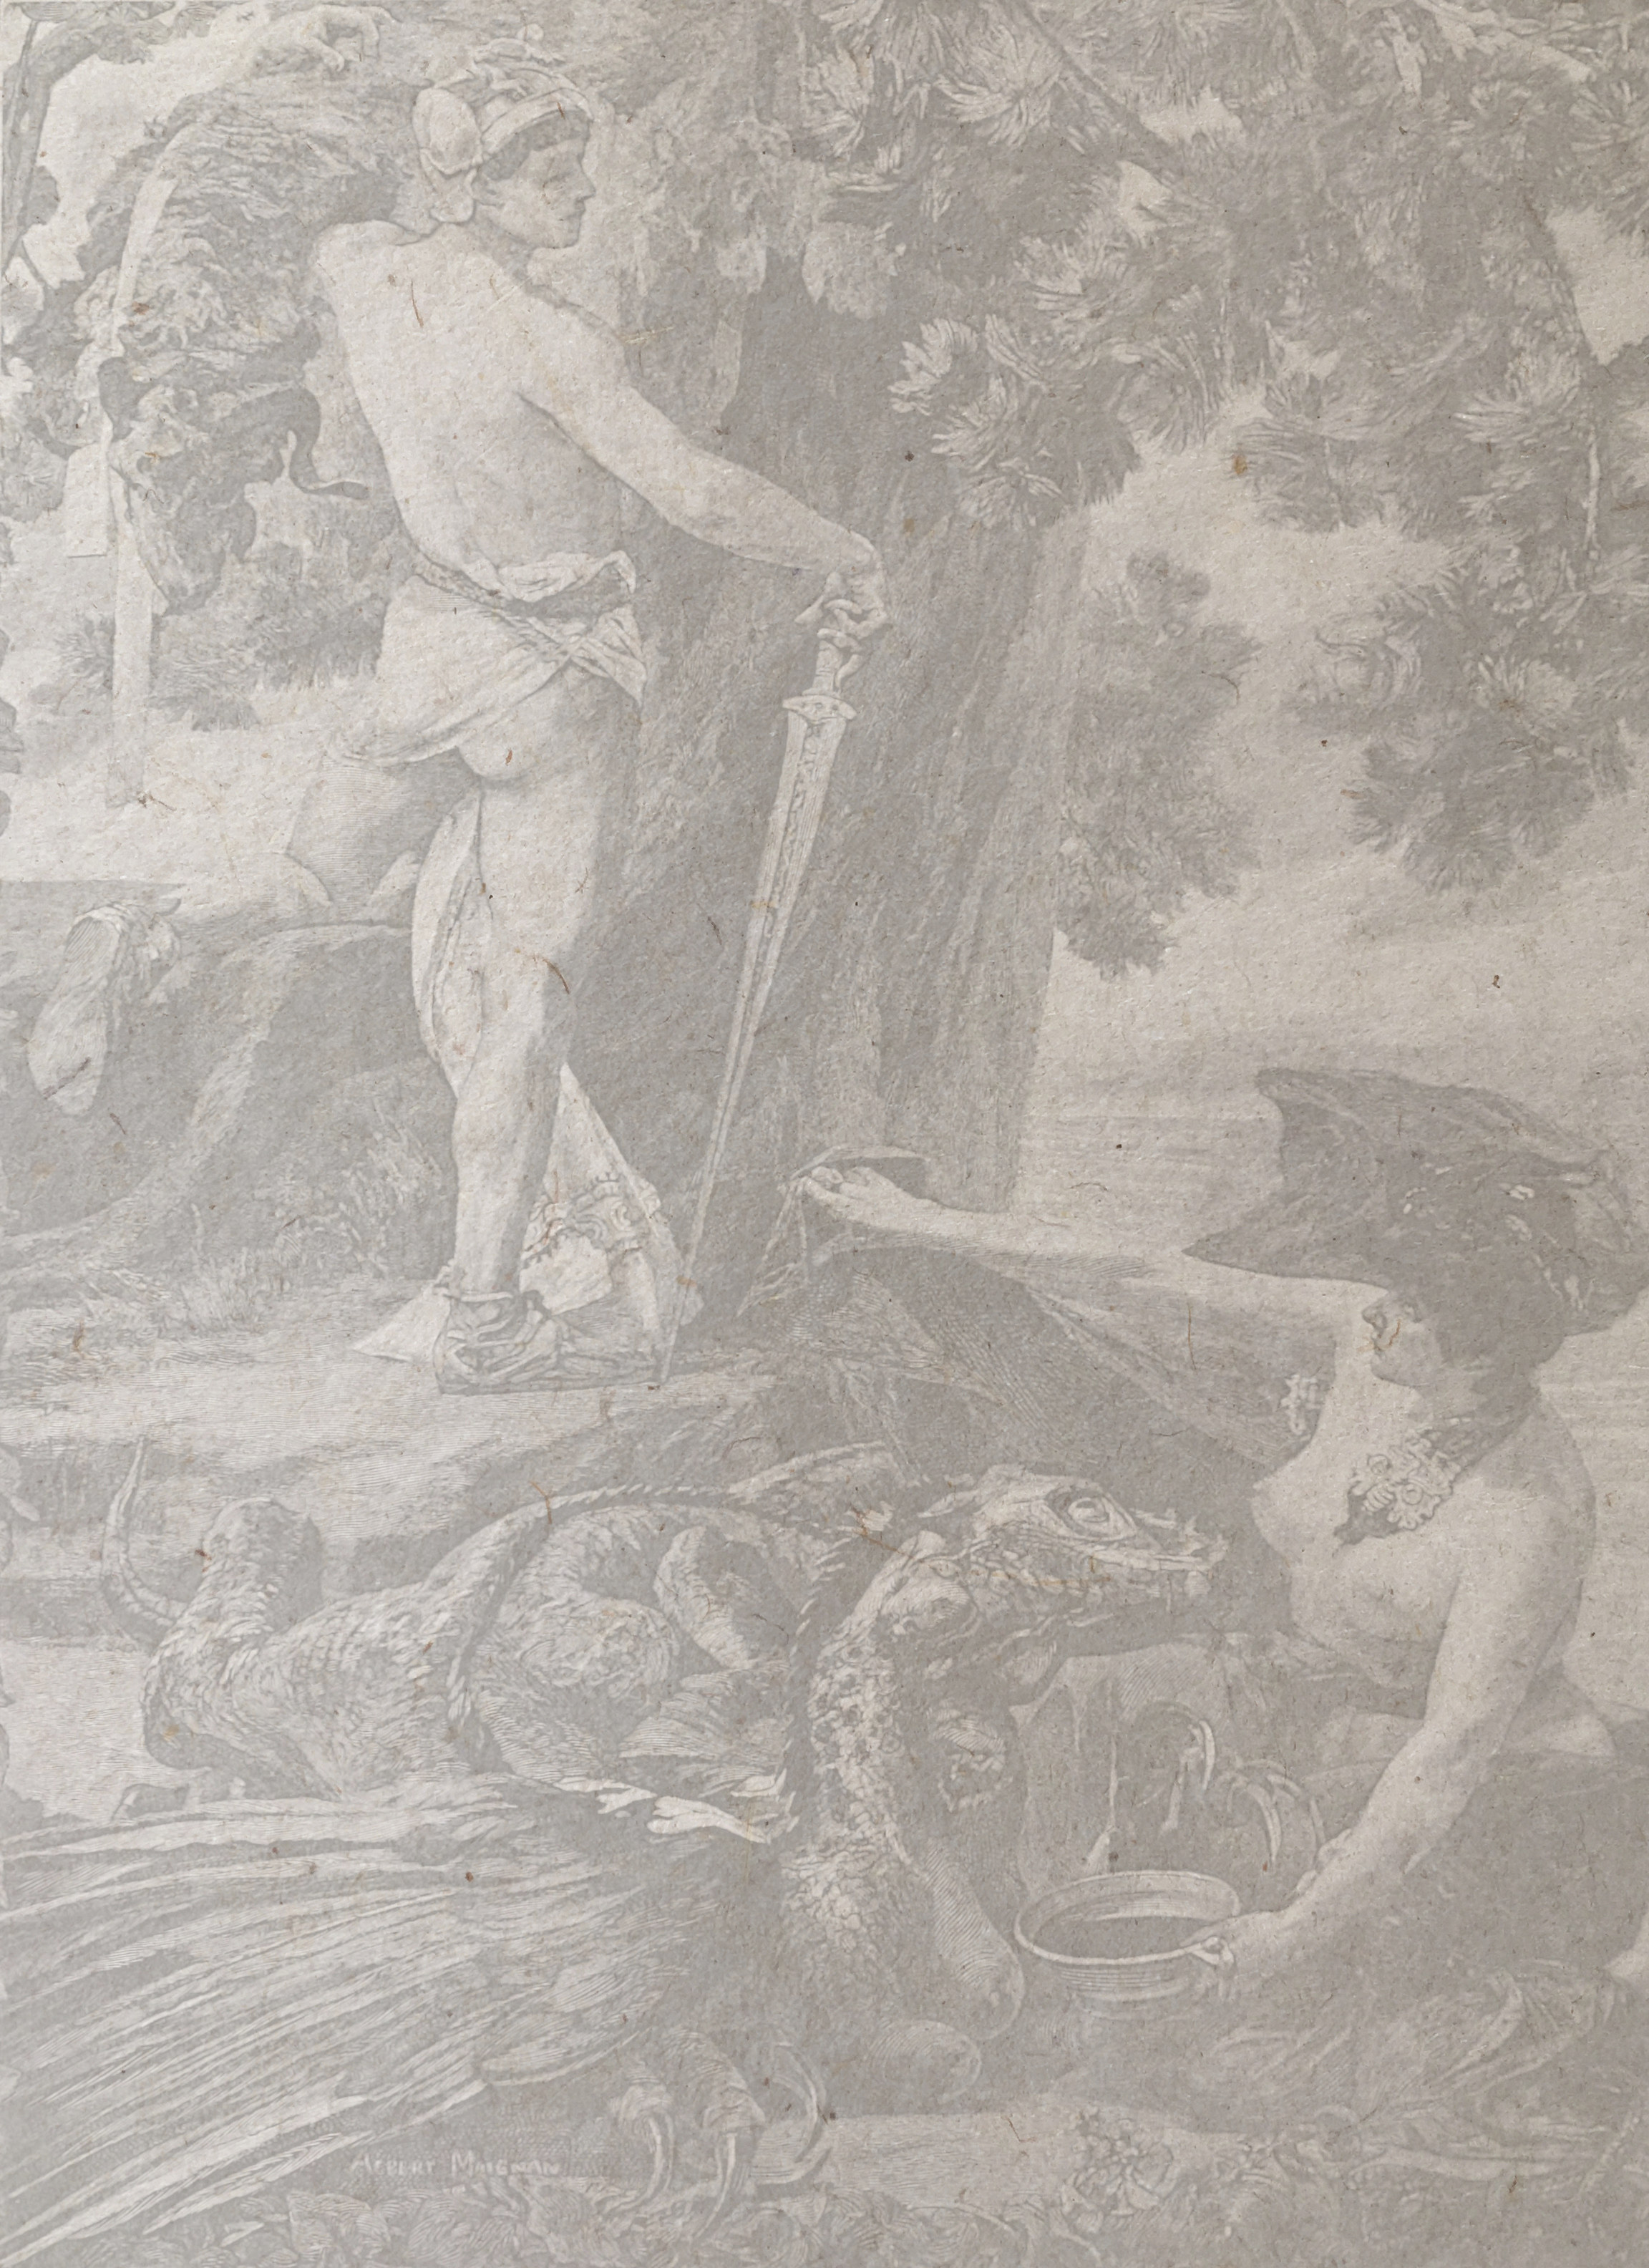
\includegraphics[width=\paperwidth,height=\paperheight]{Hemp_paper_in_Japan-canna10.jpeg}}

\renewcommand\thefootnote{{\color{BlueViolet}{\arabic{footnote}}}}
\let\oldfootnote\footnote
    \renewcommand{\footnote}[1]{\oldfootnote{{\color{BlueViolet}#1}}}
\begin{titlepage} % Suppresses headers and footers on the title page
	\centering % Centre everything on the title page
	%\scshape % Use small caps for all text on the title page

	%------------------------------------------------
	%	Title
	%------------------------------------------------
	
	\rule{\textwidth}{1.6pt}\vspace*{-\baselineskip}\vspace*{2pt} % Thick horizontal rule
	\rule{\textwidth}{0.4pt} % Thin horizontal rule
	
	\vspace{1\baselineskip} % Whitespace above the title
	
	{\scshape\Huge \textbf{De Medeae Fabula},\\ \Large Particula 2.}
	
	\vspace{1\baselineskip} % Whitespace above the title

	\rule{\textwidth}{0.4pt}\vspace*{-\baselineskip}\vspace{3.2pt} % Thin horizontal rule
	\rule{\textwidth}{1.6pt} % Thick horizontal rule
	
	\vspace{1\baselineskip} % Whitespace after the title block
	
	%------------------------------------------------
	%	Subtitle
	%------------------------------------------------
	
	{\scshape \large Dissertatio Inauguralis Archaeologica quam Consensu et Auctoritate Amplissimi Philosophorum Ordinis in Alma Litteraria Universitate Friderica Guilelma}
 
        \vspace{0.5\baselineskip}
        
        {\scshape \small Ad Summos in Philosophia Honores Rite Capessendos die 30. M. Julii A. 1850.}

        \vspace{0.5\baselineskip}
        
        {\scshape \scriptsize H. L. Q. S. Publick Defendet Auctor} % Subtitle or further description
	
	\vspace*{1\baselineskip} % Whitespace under the subtitle
	
        {\scshape \Large \textbf{Carolus Theodorus Pyl}\\\normalsize Gryphiensis.} % Subtitle or further description

	\vspace*{1\baselineskip} % Whitespace under the subtitle

        {\scshape \scriptsize Adversarii Erunt: G. M. Lane, Phil. Stud.; C. F. Hildebrant, Phil. Stud.; B. Fr. W. Kromayer, Phil. Stud.}
	%------------------------------------------------
	%	Editor(s)
	%------------------------------------------------
        \vspace*{\fill}

	\vspace{1\baselineskip}

	{\small\scshape Berolini, 1850.}
	
	{\small\scshape{Typis Gustavi Schade.}}
	
	\vspace{0.5\baselineskip} % Whitespace after the title block

        \scshape Internet Archive Online Edition% Publication year
	
	{\scshape\small Namensnennung Nicht-kommerziell Weitergabe unter gleichen Bedingungen 4.0 International} % Publisher
\end{titlepage}
\setlength{\parskip}{1mm plus1mm minus1mm}
\clearpage
\tableofcontents
\clearpage
\bfseries
\vspace*{\fill}

D. Ottoni Jahn, Prof. Lipsiensi;

D. Antonio Urlichs, Prof. Gryphiensi;

D. Eduardo Gerhard, Prof. Berolinensi;

Viris Doctissimis Amplissimisque

Praeceptoribus Optimis

Hunc Librum Dedicat

C. Th. Pyl.
\vspace*{\fill}
\clearpage
\begin{center}
\Huge\textbf{Medeae Fabula}

\large\emph{Secundum Monumenta Artium Literarumque Enarratur.}
\end{center}
\section{Cap. 1. --- De Medeae stirpe ac patria.}
\paragraph{}
Medeae patrem Aeeten fuisse, omnes scriptores consentiunt. Mater ejus apud Hesiodum (theog. 960) Ἰδνῖα filia Oceani, apud Apollonium 3. 243 et Apollodorum 1. 9, 23 Εἰδνῖα nominatur, apud Tzetzem (ad Lyc. 174) varia lectio est Εἰδαια. Secundum Diodorum 4. 45 ejus mater Hecate est filia Persae fratris Aeetae, regia Taurici atque (Hesiod. th. 409) Asteriae. Quamobrem Hecate etiam Perseis nomiuatur. Aeetae patrem fuisse Helium, omnes scriptores consentiunt Medeae stirps igitur a Diis oriunda est. Mater Aeetae apud Homerum (Od. 10. 139) et Hyginum Perse filia Oceani, apud Hesiodum (th. 956) et Apollodorum 1. 9, 1 Perseis Oceanine appellatur. Ab Eumelo (sch. a. Pind. Ol. 13. 75) mater Antiope, secundum Argonautica, quae Epimenides scripsisse dicitur (sch. ad. Ap. Arg. 3. 242) Ephyra, secundum Orphica 1216 Asterope nominatur.

Praeter Medeam Aeetae et Idyiae filiam fuisse Chalciopam Apollonius 3. Apollodorus 1. 9, 23 Hyginus (fab. 19) retulerunt. Apud scholiastam (ad Ap. Arg. 2. 1123) Jophossa 2. 1149 etiam Euenia vel Ophiusa nominatur.

Apollodorus et Hyginus etiam retulerunt, filium Aeetae et Idyiae fuisse Absyrtum qui apud scholiastam (Eur. Med. 169) Axyrtus et in tragoedia Dicaeogenis, quae Medea inscripta fuit, Metapontius et in Timonactis Scythicis Phaeton nominatur. Secundum Diodorum 4. 45 et Pacuvium (cf. Cic. d. nat. deor. 3. 9) et Justinum 42. 3 frater Medeae Aegialus, ejusque soror Circe nominatur, quam Aeetae sororem esse Homerus (Od. 10. 139) Hesiodus (th. 957) Apollodorus 1. 9 tradiderunt. A Sophocle in Colchis mater Absyrti Neaeris vel Neaera, Medeae autem mater Idyia nominatur (cf. sch. ad. Ap. 4. 223). Ab Apollonio ipso mater Absyrti Asterodea, a scholiasta 3. 242 Eyrylyte vel Eriauge etiam Hypsea vel Ipsia appellatur, quae nympha fuisse, et ab Aeete post Idyiae mortem in matrimouium ducta esse dicitur.

Patria Medeae apud Homerum et Mimnermum Aea vel insula Aeaea, apud Eumelum et Ptolemaeum Gaea, apud Stephanum (s. v.) Dia nominatur atque sita est, ubi sol oritur. Hesiodus et Simonides terram Aeetae omiserunt, Eumelus apud scholiastam ad Pindarum (Ol. 13. 75) et Pausaniam 2. 3, 10 et Tzetzem 175 narrat, Aeeten ab Helio patre Ephyraeam terram, cui postea erat nomeu Corintho, accepisse aliquanto autem post eum terram Buno tradidisse et in terram Colchidem migrasse. Eumelus primus patriam Medeae Colchidem nominavit. Pindarus tantummodo Phasidem fluvium populumque Colchorum nigris oculis commemoravit. A posterioribus scriptoribus modo Κολχίδος γᾶς cf. Aesch. Prometh. 415. modo αἶα Κόλχις (Herod. 1. 2) modo Κόλχων αἶα (Eur. Med. 2) modo Κολχικῆ γῆ (Apolld. 1. 9, 23) modo Κόλχις et terra et urbs nominatur. Urbs a Diodoro 4. 48 Sybaris, a Callimacho apud Strabonem 1. 45 a Stephano et Tzetze 144 etiam a Propertio 2. 1, 73 Cytaea nominatur, quamobrem Colchi (Apoll. 2. 1269) Cytaei et Medea saepenumero Cytaeis appellatur. Etiam Pitye vel Pityea, cui postea erat nomen Lampsaco, urbs Aeetae nominatur (sch. Apoll. 1. 933).

Ceteri autem scriptores consentiunt Colchidem esse in extremo ponto Euxino, ubi Phasis fluvius in mare effunditur, sitam.

Apud Homerum Aeetes ὀλοόφρων ab Hesiodo autem διοτρεφής βασιλεύς nominatur. In anthologiae Graecae appendice (ed. Tauchn. 329) Aeetes Κόλχοισι πολυχρύσοισι ἄναξ appellatur. Munimenta grandia urbis, splendoremque arcis copiose Apollonius (Arg. 3. 215-240), Orphica 765 describunt, atque opes divitiasque Aeetae praedicantem Apollonius 4. 1102 Alcinoum regem Phaeacum introduxit. Animum Aeetae durum superbum iracundum fuisse omnes scriptores consentiunt. Etiam monumenta, in quibus depictus est, descriptionibus respondent. Semper regio habitu modo Phrygio modo Graeco vestimento indutus est.
\clearpage
\section{Cap. 2. --- De rebus a Medea gestis, priusquam Argonautae in Colchidem adventaverunt.}
\paragraph{}
Apollonius 3. 733 narrat, Medeam a Chalciopa sorore majore natu, quum infans esset, magno cum amore curatam et eruditam esse, deinde adulta aetate sacerdotem Hecatae factam ejusque in templo esse commoratam. Pulchritudine et venustate eam praeditam fuisse, tradiderunt Apollonius 3. 830 Orphica 795. Etiam ab Hesiodo (th. 961) ἐύσφυρος et 998 ἑλικώπις nominata est. Etiam monumenta, in quibus ejus effigies, cujusmodi hoc tempore erat, expressa est, a scriptoribus non discrepant. In illis autem monumentis, in quibus depicta est illo tempore, quo in Graecia versabatur, cum pulchritudine et venustate modo gravitas severitasque, modo magnus ardor furorque mixtus est, ut partim verecundia partim admiratione partim terrore quodam commoveamur. Cujusmodi cum picturis etiam descriptiones monumentorum, quae exstincta sunt, apud Philostratum atque in Anthologia Graeca conveniunt. Plerumque Phrygio vestimento et mitra ornata, interdum autem Graeco habitu picta est. Etiamtunc, adulta aetate Medea animoque integro quum esset, Phrixus filius Athamantis et Nephelae in Colchidem adventavit. Hic enim atque Helle soror, ne immolarentur, Orchomeno effugerant ah ariete aurei velleris, quem Mercurius iis miserat, per mare transportati (cf. Apollod. 1. 9, 1). Jam Hesiodus et Pherecydes apud Eratosthenem 19 et Mimnermus apud Strabonem p. 46 aurei velleris, atque Simonides (schol. Eur. Med. 5) purpurei mentionem fecerunt.

Arietem peperit Theophane filia Bisaltae Neptuno, qui se in arietem mutaverat (cf. Hyg. fab. 188 Ovid. Met. 6. 117). Hellen undis haustam, mareque ab ea Hellespontum esse nominatura plerique scriptores tradiderunt (cf. Apolld. 1. 9, 1. Schol. Ap. Arg. 2. 1147. Herod. 7. 58). Secundum Eratosthenem 19 a Neptuno eam servatam esse, ab eoque Paeonem filium secundum Stephanum (s. v. ἀλμωπία) Almopem secundum Hyginum (poet. astr. 2. 22). Edonum peperisse, apparet. Phrixus solus in Colchidem adventavit, ibique arietem Jovi Laphystio (Paus. 1. 24, 2) vel Phyxio vel Marti vel Mercurio sacrificavit (sch. Pind. Pyth. 4. 428). Secundum Hecataeum (sch. Apoll. 1. 256) aries ipse se ad immolandum obtulisse dicitur (cf. Apollon. 1. 763. sch. Ili. 7. 86). Secundum scholiastam (Apoll. Arg. 1. 933. 2. 181, 653) et fragmentum Hesiodi (sch. Ap. 4. 284) Phrixus arietem apud Dipsacum regem Bithyniae immolasse dicitur. Secundum ceteros scriptores aureum vellus apud Aeeten in Silva Martis in arbore affixit, deinde Chalciopam filiam Aeetae in matrimonium duxit. Hercules Phrixi amicus Athamanti patri nuntium fert, Phrixum iter feliciter fecisse, quare impedit, quominus Athamas immoletur (cf. schol. Aristoph. vespae. 256). Secundum Herodotum 7. 197 filius Phrixi Cytissorus hunc nuntium fert (cf. Sophoclis fragmenta Athamantis stephanoph. Welk. Gr. Trag.). Chalciopa Phrixo secundum Apollonium 2. 1157 et Apollodorum 1. 9, 1 peperit quatuor filios Argum, Cytissorum, Phrontidem, Melan; secundum Epimenidea Argonautica (sch. Apoll. 2. 1123, Paus. 9. 34, 5) etiam filius Phrixi fuit Presbon. In Hygini fabula 14, 19 nominantur Phronius, Demoleon vel Deilion, Antolycus, Phlogius, atque Argus, Melas, Phrontides, Cylindrus. Apud Tzetzem 310 etiam Catis Sorus et filia Helle commemorantur. --- Diodorus a ceteris scriptoribus discrepat. Phrixus enim ad regem Scytharum, generum Aeetae, venisse atque post ejus mortem imperium accepisse dicitur. Aeetes autem oraculo accepto, sibi per peregrinos nautas vellus petentes mortem destinatam esse omnes peregrinos interfecisse traditur (cf. Hyg. f. 22). Praeterea Diodorus (4. 45, 46) tradidit, Medeam Circenque sororem a matre Hecate arte venefica esse imbutas. Etiam ab Apollodoro 1, 9, 23 φαρμακίς Medea appellatur (cf. Apoll. 3. 27). Circen Diodorus pergit, ab illo rege Scytharum, ad quem Phrixus se contulit, in matrimonium ductam, tum, marito occiso, imperio potitam propter crudelitatem a civibus, imperio in Phrixum translato, coactam esse, in insulam Aeaeam vel Circaeum in Italiam effugere. Secundum Apollonium 3. 310 Aeetes sororem, Helii curru usus, in Tyrrheniam duxit. Medeam autem, Diodorus pergit, initiorem clementioremque animum habuisse eamque ob rem peregrinos, quos Aeetes, ut jam supra dixi, interficere solebat, servare ausam esse. Quam rem quum Aeetes compertum habuisset, metu patris perturbatam in templum Hecatae effugisse.

Res, de quibus adhuc egimus, compluribus picturis gemmisque illustratae sunt. (Cf. Odofredi Muell. arch. artis §. 412, 3. Tölken catal. gemmarum musei Berol. p. 270. 4. 2. 139-147.)

1, In pictura parietis Pompejana (Pitt. Erc. 3. 23 ; Mus. Borbonic. 2. 19. 6. 19; Zahn Wandg. 2.; Millin Myth. Gall. CII. 409) Phrixus chlamyde indutus ab ariete aurei velleris trans mare portatur. Helle soror crinibus solutis ex undis eminet, cui frater, ne in aqua pereat, manus frustra tendere videtur. 2, In cylice (r. Tischbein Vasgm. 3. 2. Millin M. G. CII. 408). 3, in terracotta Musei Berol. (Arch. Zeit 1845 p. 37. taf. 27). 4, in gemma musei Berol. (Tölk. 4. 2. 130.) puella chitone peploque induta ab ariete per undas transmittitur. Millin et Tölken eam Hellen appellaverunt, trajectam ab ariete aurei velleris. Accurate nec, tribus monumentis eandem personam expressam esse, contendi, nec, Hellen esse, negari potest, quoniam figurae proprio signo carent, atque, fabula exstante, Hellen a Neptuno servatam esse, conjici licet, Neptunum, ne in aqua periret, ei arietem misisse, aut ipsum ejus formam accepisse. Sed veresimilior est interpretatio Panofcae, qui mulierem Theophanen filiara Bisaltae appellavit, qui a Neptuno, forma arietis accepta, per undas trajiceretur, praesertim quum de transformatione Neptuni, ubi Hellen servavit, nulla mentio exstet.

Ceterae interpretationes, quas Bergk et Lauer protulerunt, non ad nostram fabulam pertinent. (Cf. Arch. Zeit. 4. p. 214. 5. 47). 5, In interiore parte lepastae Musei Berol. (r. Gerh. Berl. Ant. Bildw. p. 279. 996) Phrixus solus ab ariete albi velleris per undas transportatur, chlamyde indutus. Albo colore candor aurei velleris significatur.

6, In interiore parte cylicis Gerbardi (r. publ. Phrixos der Herold 2. Progr. z. Berl. Winkelm. Fest. 1842) Phrixus chlamyde petasoque indutus, manu caduceum tenente, ariete vehitur. Alii juvenem, arbitrati sunt, esse Mercurium marinum, quum caduceum manu ferret. Mercurius enim saepenumero in monumentis ariete vehitur. Sed Gerhard, quum Mercurius arietem Phrixo non solum salutis, sed etiam immolandi causa obtulerit atque caduceus modo nuntii modo sacrificii perficiendi signum fuerit, recte conjecit, juvenem esse Phrixum, cui Mercurius caduceum arietis immolandi causa tradiderit. Ad sacrificium etiam pertiuet gladius, quem Phrixus manu tenet in nummo Gelonis (Mus. d. pr. d. cast. d. Torremuzza 33. 5) ubi chlamyde indutus galeaque exstructus ariete vehitur. 8, in pictura parietis Pompejana (Mus. borbon 2. 19. 2) aries in terram Colchidem exit, in quo Phrixus chlamyde indutus recubat. 9, In compluribus nummis Gelonis (Torremuzza 33; 3, 4, 6 Paruta taf. 144) Phrixus eodem habitu, quo 33. 5. expressus est, gladioque arietem immolat. 10, Cum his monumentis descriptio exstincti signi apud Pausaniam 1. 24. 2. comparanda est. (Cf. Apollon. Arg. 1. 763) quo Phrixus illustratur, oculis in aram sacrificam conversis.

11, Maximi ponderis est pictura in superiore parte alterius lateris maximae amphorae ansis volutis in museo Berol. (cf. Raoul Rochelle mou. ined. taf. 35. p. 194. Gerhard Apul. Vasbild. Erg. taf. A. 6. p. 30. Berl. Ant. Bildw. p. 285. N. 1003).

In media pictura mulier alata, crinibus promissis, longo chitone praetexto induta, arietem candentis coloris frustra effugere quaerentem, cujus cornu altera manu tenet, gladio vulneravit, ut sanguis profundatur. In hanc mulierem oculis conversis juvenis Phrygio vestimento mitraque indutus, hastaque armatus cum juvene sedente colloquitur, qui chlamyde indutus, hasta gladioque armatus est, crinibus promissis. Ab altera parte stant duae mulieres sacrificium intuentes, manibus junctis, longis chitonibus praetextis indutae, stephanisque ornatae, alterius capite velamine texto. Prope eas stat vir robustus chlamyde indutus clava pharetaque armatus.

In collo amphorae Furiae depictae sunt Orestem fugitivum persecutae. Propterea, quod utramque picturam habere quoddam commune vinculam oportere putabat, Raoul Rochette conjecit, hoc sacrificium pertinere ad Pelopem. Etenim hic a Mercurio arietem accepit, oraculo dato, quamdiu aries servaretur, fore, ut mala ab ejus stirpe averterentur. Pelope mortuo, Thyestes Atreo fratri arietem eripuit, eaque re occasionem dedit belli.

Itaque R. R. virum Phrygio vestimento Pelopem, juvenem sedentem Orestem ejus pronepotem, mulierem alatam Eridem, virum robustum Herculem, mulieres Cererem et Proserpinam nominavit. Hoc modo tres res, quae non eodem tempore gestae sunt, in una pictura per singulos homines significantur. Primum actio arietis accepti per Pelopem, deinde actio rapinae et discordiae per Eridem arietem immolantem, denique actio discordiae finiendae per Orestem significatur, cujus fuga in collo amphorae depicta est. Verum, etsi fieri potest, ut res, quae non eodem tempore gestae sunt, non solum in una pictura sed etiam symbolice per singulas homines significentur, tamen in hac pictura haec interpretatio propterea refutanda est, primum quod Pelops eadem aetate ab artifice depictus est, qua pronepos, deinde quod nec Thyestes nec Atreus, quos primas partes agere oportet, adsunt, tum quod aries raptus quidem, verum non occisus est, denique quod non explicatum est, cur Hercules atque Ceres Proserpinaque adsint.

Quamobrem Gerhard (Apul. Vasb. p. 30) arbitratus est, sacrificium esse a fratribus factum, ut culpa Thyestae expiaretur. Itaque mulierem alatam Teleten appellavit, deam sacrificii perficiendi, juvenem Phrygio habitu Thyesten, juvenem sedentem Atreum. Hercules adest, quoniam (Paus. 5. 13. 3.) (Apollod. 2. 7. 2) Pelopi primum sacrificium funebre fecisse dicitur. Etiam haec explicatio mihi non placet. Nam primum non apparet, cur Ceres et Proserpina adsint, deinde aries illius sacrificii, cui Hercules praefuit, nigro colore esse oportebat, tum Thyestes non Phrygio sed Graeco habitu pictus sit necesse est, denique nulla fabula exstat, Atreum in gratiam cum Thyeste esse reductum.

Libentius sequor aliam explicationem Gerhardi (Berl. A. Bildw. N. 1003). Etiam hic mulierem alatam Teleten appellavit, quae arietem aurei velleris mactat, juvenem Phrygio habitu Phrixum, mulierem velamine tectam Medeam, quod major natu esset, alteram Chalciopam Phrixi sponsam. Juvenem sedentem Gerhard conjecit esse Jasonem, atque per eum et Herculem esse symbolice significatam Argonautarum expeditionem.

Hoc modo in media pictura initium actionis sacrificio arietis, ab utraque parte picturae exitus actionis per duces Argonautarum significatur. Sed, quamquam, hoc modo res disponi posse, supra dixi, tamen hic ea interpretatio rejicienda est, quod juvenis sedens cum Phrygio viro colloquitur. Praeterea annotandum est, Phrixum non Phrygio, sed Graeco habitu expressum esse oportere, atque Chalciopam (Apoll. 3. 734) majorem natu esse Medea.

Mea interpretatio est haec. Primum hanc picturam cum Oreste, qui in collo amphorae depictus est, cohaerere nego, deinde dico, eam ad arietem aurei velleris quidem pertinere sed alio modo, quam Gerbard interpretatus est. Ego enim juvenem sedentem Graece habitu Phrixum appello cum Absyrto, fratre uxeris, Phrygio habitu colloquentem. In media parte Telete Phrixi jussu Jovi Laphystio arietem inmolat. Ab altera parte stat Chalciopa, cujus velamen ad nuptias Phrixi pertinet, prope eam Medea minor natu. Hercules adest, ut Athamanti patri Phrixi nuntium ferat, filium iter feliciter fecisse.

Praeterea Phrixi effigiem expressam esse multis gemmis musei Berolinensis aliisque (cf. Tölken cat. p. 71. 2. 2. 139, p. 270. 4. 2. 141-148; Flangiui Apoll. Arg. 1. 434 ; Miliin M. G. 146. 424; Impronte gemm. d. inst. 1. 75. 76. 6. 32; Tassie Raspe cat. 8634-42; Niederl. M. 845-46; Lond. 557) contendo, in quibus secundum descriptionem Tölkeni aliorumque Jason fictus est, qui aureum vellus rapit. Sed quoniam Medea, ubi Jason hanc rem gerit, adsit, necesse est, in omnibus autem gemmis Jason solus eodemque modo indutus et armatus est, quo Phrixus in nummis Gelonis, deinde quum in gemmis (Millin 424. Tölken 142. 143. 147) ara cum capite arietis, et in gemmis (Tölken 144. 145) aries ipse prope aram stat, utraque autem res ad Jasonem pertinere nequit, contendere audeo, hunc juvenem esse Phrixum, qui in gemmis 144. 145. arietis immolandi consilium cepit, in ceteris autem, sacrificio facto, vellus in arbore vel in columna 144-146 affixit, quae a dracone custodita est. Huc accedit, quod Pausanias 1. 24. 2, ut jam supra dixi, signum descripsit, in quo Phrixus oculos convertit in victimam flammis combustam, quod gemmis 142. 143. 147 specimini propositum fuisse videtur. Avis, quae in gemmis 144-146 in columna sedet, ab interpretatoribus iynx appellatur. Quum Jasonem esse juvenem negaverim, haec avis non apta est ad dispositionem signi. Itaque ego arbitror, cornicem esse vaticinio praeditam, a qua Phrixus mandatum Mercurii accepit arietis immolaudi.

Cujusmodi cornices in silva Martis, ubi aureum vellus ab arbore dependebat, fuisse Apollonius 3. 930 tradidit.
\clearpage
\section{Cap. 3. --- De Medea Argonautarum adjutrice.}
\subsection{De Jasonis stirpe ac patria.}
\paragraph{}
Argonautarum expeditio brevissime ab Homero Hesiodo Minmermo commemoratur. Jason, quem ducem eorum fuisse plerique scriptores consentiunt, fuit secundum omnia scripta monumenta filius Aesonis, de cujus stirpe Homerus (Od. 11. 235) tradidit. Mater ejus apud Apollonium 1. 232 et Hyginum 14 Alcimede ab Apollodoro 1. 9, 16 Polymede, ab scholiasta (Od. 12, 70) Polymele, a Diodoro 4. 50 Amphinome, a scholiasta (Apoll. Arg. 1. 45, 230) Periclymene et Polypheme, a Stesichoro Eteoclymene, a Tzetze (ad Lyc. 872) Arne vel Scarphe (Chiliad. 7. 980) Rhoeo appellatur. Frater Jasonis Promachus ab Apollodoro 1. 9, 27 et Diodoro 4. 50 commemoratur, sororem Hippolyten Odofredus Mueller (in tert. append. Orchomeni) profert, cujus mentionem praeterea non inveni. Apollonius 1. 288 contra tradidit, Aesoni Jasonem solum ab Alcimede esse partum.

Patriam ejus Jolcum ad Pagasaeum sinum in Thessalia fuisse omnes scriptores consentiunt. Jasonem a Chirone in Pelio monte educatum esse Pindarus et Hesiodus (sch. P. Nem. 3. 92) tradiderunt. Etenim quum Pelias frater Aesonis, oraculo accepto, mortem sibi ab Aeolide destinatam esse, Jasoni insidias paravisset, ejus propinqui Peliam mendaciis, puerum periisse, fefellerunt, ipsum autem arcano ad Chironem duxerunt. Antea Diomedes appellatus esse, a Chirone antem ei nomen Jason datum traditur (cf. Arch. Zeit. 1845 p. 178; Natal. Com. 6. 8; Bull. 1838, 13). Sed quam adolevisset, vestimento Magnetum indutus hastisque armatus ad patrem reversus, a Pelia qui regno potitus est, imperium repetivit. A Pindaro abhorret Pherecydes (schol. Od. 12. 70). Nam, Aeson postquam mortem occubuit, a Pelia tutore imperio suscepto, Jason agram prope Anauram fluvium coluisse dicitur (cf. Apoll. 1. 9. Hygin. 12). Quondam, quum Jason, ut sacrificio Peliae adesset, fluvium transiret, eum unum calceum amisisse, Apollodorus 1. 9, 16 tradidit. Secundum Hyginum (f. 13) et Apollonium 3. 70 calceum amisit, ubi Junonem, quae se ad eum contulerat, quod, ut jam Homerus (Od. 12. 69) narravit, amore ejus incensa erat, trans Anaurum vel Enipeum vel Euenum fluvium transportavit. Pelias autem, altero oraculo accepto, cavendum esse a monocrepide, quum Jasonem conspexisset, metu ejus perturbatus secundum Pindarum et Apollonium 3. 338 eum jussit aureum vellus reportare ut manes Phrixi expiarentur. Secundum Apollodorum 1. 9. 16. Jason interrogatus, quomodo se in eum gereret, a quo sibi mors immineret, Peliae respondisse dicitur, se mandatum ei daturum esse, aurei velleris reportandi. Tum Pelias ei hoc mandatum dedisse traditur.

Diodorus 4. 40 narravit, Jasoni, cujus animus magnis a majoribus rebus gestis inflammatus esset, a Pelia, quem audacia juvenis timore implevisset, persuasum esse, ut, animo satisfaciendi causa, aureum vellus reportaret. Hesiodus (th. 995) nullam causam expeditionis annotat, nisi Peliae insolentiam. Tum Pindarus pergit, Junonem Pelasgicam quae secundum Apollonium 2. 14. 3. 1135. 4. 243. Peliae succensuit, quod sacrificium ejus neglexisset, Jasonem magno animo implevisse et effecisse, ut navis Argo aedificaretur. In Orphicis 60 animus ejus demissus et perculsus ab ea relevatur. Apud Apollonium 1. 19 Argus filius Arestoris vel Alectoris (Diod. 4. 41) apud Apollodorum 1. 9, 16 Argus filius Phrixi navem aedificat. Apud Athenaeum (7. 12. p. 296) (cf. Welk. Tril. 311) Glaucus, apud Ptolemaeum (Heph. 2) Hercules nominatur. In Orphicis 66 jubet Inno Minervam Tritogeniam navem exstruere (cf. Val. Flac. 1. 305) et partem quercus Dodonaeae sermone praeditam adjungere (cf. Apoll. 4. 580, 1. 525; Orph. 265; Flacc. 1. 302; Apolld. 1. 9, 16). Hercules postquam munus ducis recusavit (Apoll. 1. 340; Hyg. 14; Orph. 300) Jason dux creatur, atque posteaquam parentibus Aesoni et Alcimedae (Apoll. 260-300) tum Iphiae seni sacerdoti Dianae (313) denique Chironi de Pelio monte descendenti (553. Orph. 380) valedixit, atque Apollini Pagasaeo (360) Diisque marinis (Orph. 330) sacrificavit, cum Argonautis navem conscendit.

Secundum Dionysium (ap. Appolld. 1. 9. 19) et Diodorum 4. 41, qui illum secutus esse videtur, Hercules dux Argonautarum est. In Aretia insula (Ap. 2. 1120) Jasoni occurrunt filii Phrixi, Argus, qui apud Apollodorum 1. 9, 16 navem aedificaverat, Cytissoros, Phrontis, Melas, qui patris jussu post ejus mortem, ut hereditatem caperent, Colchide reversi atque naufragio ad insulam delati sunt. Jason quamvis eum moneant, Aeeten esse cavendum, tamen cum iis Colchidem iter persequitor.

Secundum Hyginum (f. 3, 1 Mythol, ed. Bode 23) Phrixus ab Aeete occisus est, secundum Pausaniam 9. 34, 3 ipse Orchomenum reversus, secundum Apollonium (2. 1151. Orph. 794) apud Aeeten morbo exstinctus est.

Jasonem pulchritudine et venustate ceteris Argonautis praecelluisse, non solum scriptores consentiunt (cf. Apoll. Arg. 1. 775. 3. 956. Orph. 806) sed etiam ex monumentis, quae exstant, atque ex descriptione deperditorum apparet. In plerisque monumentis Jason imberbis adulta aetate chlamyde indutus exprimitur. Interdum barbatus et virili habitu, etiam more Magnetum (cf. Pind. Pyth. 4) indutus est. Cum illo habitu descriptio Philostrati jun, 7. convenit: ἰούλῳ τε ἤδη βρύει καθέρποντι καί ἡ κόμη ξανθὴ ἐπισάλευει τῷ μετωπῷ.

Jasonis effigies statua illustratur, quae, priusquam Winkelmann eam illustraret, Cincinnatus nominari solebat, quia restaurator ineptus aratrum adjunxerat (cf. Description d. mus. Roy. 1830. N. 710; Maffei Raccolt. d. stat. ant. 70; Mus. d. ant. par Bouillon. 2. 6; Mus. franc. par Rohil-Peronville et Laurent. 3. 15; Clarac Mus. d. Louvre p. 309, capite antiquo ab altera statua adjuncto, cf. Visconti M. Pioclem 7. p. 101; Cop. e Hadriani villa Tiburtina in museum Monac. portata, Beschr. Glypt. Kleuze u. Schorn. 150; in Britanniam portata; cf. Bött. Amalth. 3. p. 242 in shelnburnhouse; cf. Goede Reis. in Engl. 4. p. 43 in Landsdownehouse; cf. mus. cap. 3. 51; similis statua minor invenitur cf. Pioclem. 3. 48; mus. franc. 3. 48; Clar. pl. 814 O. M. Arch. d. K. §. 157, 3; Millin M. G. CII. 416). Juvenis chlamyde indutus pedem in lapide posuit, ut calceum sibi in duceret. Alter calceus juxta lapidem situs est. Ocoli juvenis a calceis aversi sunt. Winkelmann, quum aratrum falso esse adjunctum appareret, jnvenem Jasonem appellavit, cujus oculi ad Junonem conversi essent, quae supplex adventaret, ut trans fluvium trajiceretur, quo fieret, ut alterius calcei inducendi oblivisceretur. Visconti annotat (cf. Stuart 2. ch. 1. pl. 30 A.) duos viros eodem situ in Partheno esse expressos. Odofredus Mueller (§. 157, 3) arbitratur, fere eodem tempore hanc statuam esse fictam, quo gladiatorem Borghesianum.

Aedificatio navis multis anaglyphis fictilibus, ex quo numero una in Museo Berol. invenitur, illustratur. 1. Minerva duos viros barbatos, chitonibus indutos navem aedificantes adjuvat. Alter vir galea armatus est. Eodem modo armatus 2. in anaglypho aeneo vir barbatus navem aedificat, quocum Minerva et Mercurius colloquuntur (cf. ad. 1 et 2. Flangini. Ap. Arg. Taf. 1. 2; Winkelm. Mon. Ined. 1; Millin G. M. 130. 417, 105. 418; O. Muell. D. A. K. 2. 22. N. 238; Combe terrae. Br. M. pl. 10. N. 16; Campana oper. d. plast. taf. 5; Zoega bass. 45). 3. In gemma Tusca (Micali stor. 116, 2) vir barbatus navem aedificans inscriptione EASUN illustratur. 4. Simili modo vir barbatus in gemma coll. Pourtales (Impr. gemm. d. inst. 3. 64) insculptus est, sed inscriptione caret.

In anaglyphis Minerva adest, quoniam vel sua sponte vel Junonis jussu navis aedificationi praefuit. Mercurius adest, quia Deo, qui Phrixo arietem miserat, reportatio aurei velleris curae maximae sit, necesse est. Viros galea armatos in gemma Cab. Pourt. et anaglypho aeneo (cf. Mill. M. G. 105. 418) atque alterum virum barbatum in anaglypho fictili (Millin G. M. 130. 417) Millin et O. Mueller Argum appellaverunt. Sed filius Alectoris esse videtur, quum Argus Phrixi adulta aetate exprimi soleat. Alterum virum in anaglypho fictili Millin appellat Tiphyn, O. Mueller servum Argi. Hunc Jasonem appello primum, quod in Tusca gemma eodem modo fictus est, deinde quod secundum Apollonium 1. 724 etiam Jason ipse, Minerva adjuvante, navem exstruendam curavit. Aedificium in posteriore parte anaglyphi templum Pagasaei Apollonis esse, cui Jason sacrificium fecit, Millin ingeniose conjecit.

Navis undis vecta ficta est in anaglypho et nummo (cf. Flangini 1; Millingen Peint. vas. gr. div. coll. 52; Millin M. G. 105. 419; 111. 420; cf. Pausan. 1. 18, 1, ubi Argonautarum expeditionem a Micone pictam commemorat).

Aliae res ab Argonautis, antequam advenerunt Colchidem, gestae et monumentis illustratae (cf. O. Mueller Arch. §. 412, 4) omittendae sunt, quod ad Medeam non pertinent. Uno autem verho annotare volo duas picturas (cf. Cab. Dur. 256, 257) ubi Jasonem hastâ armatum coram Mercurio libantem inscriptione ASON atque 257 loricatum coram nudo adolescente inscriptione EASON illustratum conspicimus.

\subsection{De Argonautarum adventu apud Aeeteu.}
\paragraph{}
De hac re jam Pindarus brevem mentionem fecit. Copiosius Apolloniua 3. 166-395 narrat, nave ad Circaeum appulsa 200 Jasonem cum filiis Phrixi ad Aeetae aedes se contulisse 210-30 earumque magnitudinem splendoremque, fontesque quatuor ante portam 222 admiratos esse. Prima iis occurrit 255 Chalciopa filiosque laeto animo excipit, deinde 268 Aeetes, Idyia cum Medea ex aedibus egrediuntur. Nepotes ab Aeete interrogati, cur reversi essent, respondent, Argonautas venisse aurei velleris reportandi causa. Tum Aeetes magna iracundia, atque timore, ne, quae praedicta sint, eveniant, commovetur, Jason autem efficit, ut simulet, iram esse placatam. In Orphicis 775 Juno effecit, ut Aeetes in somno conspiceret Medeam prope Phasidem fluvium rapi eaque re sibi magnum malum afferri. Quamobrem mane rex cum filiis, ut malum sacrificiis averteret, curru ad fluvium vectus, Argonautis in terram egressis obviam it, atque postquam causam expeditionis compertam habuit, minis eos insequitur. Diodorus 4. 46 narrat, nave prope templum Hecatae appulsa, Argonautas Medeae obviam esse, quae in illud templum metu patris effugit.

Adventus Argonautarum praeclara pictura in superiore parte alterius lateris maximae amphorae Rubinae, quae nunc in museo Monac. invenitur, illustrata est (cf. Monit. d. 2. Sic; Dub. Maisonneuve 44).

Pictura in tres partes dispertienda est. In media parte senex calvus, barbatus, peplo indutus, manu sceptrum tenente, ab juvene laureato, nudo, gladio hastaque armato tesseram, in qua ΣΙΣΥΦΟΣ inscriptum est, accipit. Ante pedes senis hydria sita est. Altera pars picturae a media columna ionica separatur. Mulier chitone longo praetexto induta, capite velamine tecto stephaneque ornato, cum quinque juvenibus laureatis, chlamydibus indutis, hastisque armatis colloquitur, quorum vultus laetitia exhilarantur.

In altera parte mulier provecta aetate cum virgine, cujus manus supra pectus junctae sunt, colloquitur. Utraque longo chitone praetexto, velamine stephaneque ornata est, vultu significante, ut animus valde commotus sit.

Odofredus Mueller hanc picturam (Arch. d. K. §. 412, 4) brevissime explicavit: Ankunft der Argonauten bei Aietes; einer bringt ihm eine gastliche Tessera von Sisyphos in Bezug auf Aietes korinthische Herkunft; Jason und Medea schliefsen ihr Liebesbündniss. Juvenem igitur proxime mulierem Jason em appellat cum Medea coram quatuor Argonautis sponsalia facientem. Quilibet Argonauta epistola Sisyphi Aeetae iram mitigat. Hydria autem duaeque mulieres non explicantur.

Panofka igitur hanc explicationem (Arch. Zeit. 2. p. 256) refutavit, atque res apud Phaeaces esse gestas conjecit. Senem igitur Alcinoum appellavit, cui Glaucus Argonautarum gubernator epistolam Sisyphi tradit, ut regis gratiam facilius conciliet. Mulierem senem Areten appellavit quae cum Medea mundo nuptiali ornata colloqueretur. In altera parte Nausicaa coram quatuor Argonautis Jasonem certiorem facit, nuptias ejus et Medeae parandas esse, ne Colchis eam persecutis tradatur. Panofka arbitratus est senem appellari non posse Aeeten propterea, quod Graeco habitu sit. Verum in anaglyphis marmoreis (cf. Beger spid. ant. 118. Clarac 199) eodem Graeco habitu fictus est. Panofkae interpretatio autem rejicienda est primum quod Medea nuptiali mundo caret, eodemque modo indutus est, quo ceterae mulieres, deinde quod mulier cum juvene colloquens major natu est, quam ut Nausicaa esse possit, tum quod hospitium non ab gubernatore navis, sed a duce expeditionis appetatur necesse est, deinde quia inter tres tam arcte in una pictura conjunctas res nulla continuatio seriesque reram est, atque preces hospitii et nuptiarum apparatus uno tenore nec cogitari nec pingi possunt, tum quod adventus Colchorum, quae est res maximi ponderis, nulla re significatur. Cogitari quidem potest, juvenem, qui Glaucus nominatus est, esse Absyrtum aliumve ducem Colchorum, qui Medeam persecuti sunt, praesertim quum epistola Sisyphi, quoniam Aeetes Corintho oriundus est, non inepta sit. Sed hanc rem Panofka probare nequit, quod Phrygio habitu caret. Praeterea hydria non explicatur, denique haec pictura cum pugna Jasonis cum dracone cohaeret, quae in inferiore parte amphorae depicta est, atque cum nuptiis apud Phaeaces nullo modo cohaerere potest. Equidem igitur censeo, res, ut jam Odofredus Mueller conjecit, apud Aeeten esse gestas atque hanc interpretationem propono.

Jason cum filiis Phrixi ad Aeetae aedes adventavit, quae ionica columna significantur. Ad fontes ante portam hydria spectat. Mulierem prope columnam Chalciopam appello cum filiis colloquentem. Propterea, quod mater prima iis occurrit (cf. Apoll. 3. 255) vultus eorum gaudio commoventur. Juvenis, qui Aeetae epistolam tradit Jason est. Etenim primum boc munus debetur duci, deinde etiam Apollonius, quem pictor secutus esse videtur, tradidit a Jasone iram Aeetae esse mitigatam. Epistola Sisyphi haec res effici potuit, quoniam et Jasonis et Aeetae propinquus erat. Mulieres appello Idyiam et Medeam. Haec pulchritudinem Jasonis admirari, mater autem hortari videtur, hospitem esse cavendum.

\subsection{De amore inter Medeam et Jasonem.}
\paragraph{}
Secundum Pindarum Venus Medeam vi magica iyngis avis incantamentisque amore Jasonis inflammavit, apud Apollonium 3. 280 ff. Medea, Junonis Venerisque jussu, Amoris sagitta vulneratur (cf. Orphic. 867). Apud Valerium Flaccum 7. 347. Juno et Venus, specie Chalciopae et Circae accepta, blandis verbis efficiunt, ut. Medea amore Jasonis inflammetur. Apud Hyginum 21. 22. Juno Medeae somnianti Jasonem monstrat, cujus pulchritudine amor Medeae incenditor.

Tum, ut Pindarus pergit, Aeetes Jasoni aureum vellus cum hac conditione promisit, ut ignivomos aeripedesque boves, quos Vulcanus ei dederat, aratro adjungeret, iisque terram araret, ut ceteri scriptores addunt, etiam dentes draconis sulcis imponeret, atque cum viris ex iis oriundis manus consereret. Aeetes enim secundum Apollonium (3. 1182. Apoll. 1. 9. 23. Serv. ad Georg. 2. 141) a Minerva dimidiam partem dentium draconis a Cadmo occisi acceperat. Aeetes has conditiones, quibus neminem satisfacere posse putabat, praescripsit, quod, ut jam supra dixi, oraculum acceperat, quamdiu vellus in silva Martis penderet, fore, ut imperium obtineret. (Cf. Hyg. f. 22). Jam Hesiodus (th. 994) de magnis pugnis Jasonis mentionem fecit. Jason secundum Apollonium conditiones animo demisso suscepit, Argum filium Chalciopae ad matrem misit quae Medeam persuaderet, ut sibi magica arte opitularetur In Orphicis 860. Medea ipsa Argum, qui Colchidem in hoc carmine nondum reliquit, ad Jasonem mittit, ut eum certiorem faciat, se auxilium ei ferre velle. Tum secundum Apollonium Medeae, post longam animi contentionem amore patriae devicto, a Chalciopa persuadetur, ut Jasoni auxilium ferat. Denique cum servis ad templum Hecatae se confert, atque secum arcam portat 3. 800 in qua unguentum posuerat e herba paratum, quae ex Promethei cruore oriunda erat. Interea, ea fidibus canente, 900 Jason ab Argo certior factus ad templum venit.

Post longum sermonem amatorium, postquam Jason promisit, se eam in matrimonium ducere velle, Apollonius eodem modo, quo Pindarus narrat, Medeam docuisse eum unguento magico usum vi boum vulnerari non posse, atque si viri armati e dentibus draconis enascerentur, lapidem iuter eos jaciendum esse, quo facto fore ut ipsi manus inter se conserentes perirent. Fere eodem modo rem ceteri scriptores tradiderunt. Apud Apollodorum 1. 9. 23 Medea a Jasone petit, ut fidem jurejurando astringat. Apud Valerium Flaccum Juno et Venus, specie Chalciopae Circaeque accepta, Medeam, Iris, utriusque Deae jussu, Jasonem ad templum Hecatae ducunt. Diodorus ab omnibus abhorret 4. 46. Nam Jasoni nec conditiones ab Aeete praescribuntur, nec mentio fit boum, sed Medea fugitiva postquam Argonautis obviam ivit, atque Jason jurejurando Medeae jussu affirmavit, se eam in matrimonium ducere velle, iis promittit, se noctu dolo efficere velle, ut aureum vellus capiant.

Amor atque conventus primus Medeae et Jasonis permultis monumentis illustratur.

1. Iyngem in anaglypho fictili, quam Combe (terrac. br. Mus. 28. 53) publicavit, fictam esse, O. Mueller conjecit. Virum sedentem galea gladioque armatum cum juvene colloquentem, cujus manus caveam in lapide positam, in qua avis inclusa est, attingit, Combe Alexandrum magnum nominavit, oraculum ab Apolline petentem, avem esse cornicem Deo sacratam. O. Mueller eum Jasonem appellavit a Mercurio iyngem donum Veneris accipientem. Sed ipse hanc sententiam refutavisset, si idem anaglyphum apud Campanam (oper. d. plast. 19) accuratius designatum conspexisset. Etenim quum in hac publicatione juvenis laureatus sit, ejusque ad pedes fides ad stipitem alligatae sint, apparet juvenem Apollinem esse. Jamque ab interprete haec explicatio, quam sequimur, addita est: Aeneam esse ab Apolline, cujus vis vaticinandi corvo significatur, oraculum petentem. (Cf. Hyg. 251). 2. Contra iyngem pictam esse in vasculo, quod nunc Vindobonae invenitur, contendo (Alex. Laborde coll. d. vas. gr. de C. Lamberg 2. 3). Mulier alata, chitone induta, in columna ionica insidens juveni chlamyde induto hastaque armato avem offert. Conjeci, juvenem esse Jasonem, cui per Iridem nuntiam Deorum Venus iyngem avem mittit, ut ejus vi sibi amorem Medeae conciliet. Habitus juvenis et mulieris alatae ejusmodi est, ut ad Jasonem et Iridem accommodatus sit. Etiam non offendit, Iridem loco Veneris avem Jasoni tradere. Difficilior autem quaestio est, utrum avis iynx sit necne. Namque quum perpaucis fabulis iynx illustretur, raro sine ulla dubitatione coutendi potest, in qua pictura haec avis depicta sit. Copiose de iynge scripsit Otto Jahn, (Peitho die Göttin der Unterredung Programm zum Winkelmannsfest in Greifswald 1846 p. 14. ff. p. 28. Anm. 121) atque demonstravit, primam ejus mentionem Pindarum fecisse, ubi de nostra fabula egit, deinde alteram fabulam esse traditam: iyngem nympham, cujus mater Peitho nominatur, Jovem amore aut sui aut Jus inflammasse eamque ob rem ab Junone irata in avem mutatam esse. Nicander Metamorphoseon 4. apud Antoninum Liberalem (transform. 9) narravit, filiam Pieri fuisse atque cum Musis certamen musicum inivisse, devictam autem ab illis propter superbiam in avem esse transformatam vi amoris excitandi praeditam. Ceteros scriptores, qui ejus magicam vim atque usum commemoraverunt, Otto Jahn protulit. 3. Itaque Gerhard (Berl. Ant. B. p. 261. N. 902) avem longa cauda, quam Venus manu fert, ubi Juppiter Jus amorem appetit, iyngem appellavit, deinde 4. illa avis, quam mulier tenet (B. A. B. 1020) ubi Paris judicium fert, tum illa avis, 5. quam Pitho manu attingit (bass. Neap. Winkelm. M. J. 115; Millin G. M. 173. 540; Inghirami gall Omer. 10; Guigniaut rel. d. ant. 246. 751; Mus. Borh. 3. 40) ubi Paris ad Helenam se confert, denique 6. illa avis, quae ante pedes Calypsus sita est (Millin. G. M. 114. 444; Peint. d. vas. 1. 3) per quam draco consopitur, iynx appellatur. Sed ex his exemplis definite constitui nequit, cujusmodi effigies avis fuerit. Nam ejus forma vario modo expressa est. Longa igitur cauda non est propria et singularis nota iyngis. In nostra pictora forma avis fere anseris vel gruis esse videtur, cujusmodi altera avis ad pedes Calypsus depicta est.

Quapropter contendere audeo, formam iyngis, partim quia perpaucae fabulae de ea exstant, partim quod ejus magica vi ubique et semper usi sunt, non fuisse definitam ac singularem atque pictores, ubi avis vi amoris excitandi praedita adesset necesse erat, eam vario modo pinxisse.

Apollonium, ex quo Medeae amorem Jason non iynge sed Chalciopa illi persuadente, sibi reconciliavit, ille pictor secutus esse videtur, quem, jam supra diximus, Phrixi sacrificium in amphora musei Ber. pinxisse. Pictura in inferiore parte amphorae in tres partes divisa est. In altera parte sedet mulier longo chitone praetexto induta, capite velamine diademateque tecto, cujus ad sellam clypeus et hasta posita sunt. Altera manu sublata juvenem chlamyde indutum, hasta et clypeo gladioque armatum admonet. In media parte Minerva in suggestu sedens cum juvene colloquitur chlamyde induto, gladioque armato, qui speculum manu tenet. In tertia parte duae mulieres longis chitonibus praetextis indutae stephanisque ornatae colloquuntur, quarum vultus animum earum vehementer esse commotum, significant. Raoul Rochette (Mon. ined. taf. 35. p. 194) etiam hanc picturam ad stirpem Pelopis pertinere contendit. Mulierem sedentem appellat vel Dicen vel Areteu, quae Orestem admoneat, ut se Athenas conferat, ihique expietur. Athenas, arbitratur, significari per Minervam et per juvenem, cujus speculum ostendat, hominem esse sacratum. Mulieres colloquentes, ut in superiore pictura, Cererem et Proserpinam appellat. Sed, cur Deae adsint, non explicat. Gerhard in ea interpretatione, secundum quam in superiore parte Atreus et Thyestes in gratiam redeunt, juvenes Agamemnonem et Menelaum appellat. Uterque a Dice et Minerva ad fortitudinem admonetur. Agamemnon arma cepit, quoniam gloria helli praecelluit ceteris, Menelai speculum significare dicitur, eum mollioris animi atque maritum Helenae esse. Mulieres Clytaemnestra et Helena eorum uxores appellantur. In altera interpretatione Gerhard (B. A. B, 1003) arbitratus est, picturam pertinere ad vitam domesticam; uterque sponsus sponsaque in templum Minervae et Dicae ingressi supplices esse dicuntur, ut nuptiae sint felices. Jamque quum superiorem partem amphorae alio modo explicaverim, etiam has interpretationes rejici oportet, egoque hanc explicationem propono.

Mulierem sedentem venerabili vultu appello Junonem, juvenem armatum Jasonem. Posteaquam Aeetes ei conditiones praescripsit ad Junonem fautricem Deam se contulit (cf. Orph. 60), quae eam ad fortitudinem admonet, armisque instruit. Minerva Argum, quem jam navem aedificantem adjuverat, adhortatur, ut arma capiat, quae ad Junonis sellam sita sunt, atque matri persuadeat, ut Medea Jasoni auxilium ferat. Haec res in tertia parte illustrata est ubi easdem mulieres depictas esse, quae in superiore pictura inveniuntur, jam Raoul Rochette intellexit. --- Chalciopa enim Medeae sedenti persuadet, ut Jasoni opituletur.

Tali modo in superiore parte amphorae adventu Phrixi, arietisque sacrificio initium expeditionis Argonautarum, in inferiore parte Jasonis adventu, Medeae persuasioneque exitus rei illustratur. Difficilior quaestio est, cur Argus speculum manu teneat. Plerumque, ubi speculum invenitur, est feminis ornatui, sed saepenumero, ubi juvenis prope sepulcrum speculum tenet, vel mulieres aqua in ferentes apud inferos speculo utuntur, ornatui esse non potest. Plerumque interpretes dixerunt, instrumentum esse mysticum, sed non addiderunt, quod significaret. Significatio speculi perspicua est, ubi in pictura (R. R. Mon. ind. taf. 36. p. 187) Oresti furia, persecuta eum, speculum ante oculos ponit, in quo facies mulieris conspicitur. R. R. et O. Mueller recte conjecerunt (Arch. d. K. §. 398, 5) faciem esse Clytaemnestrae, qua Orestes parricidii reminisceretur.

Tali modo apparet, speculum mysticum significare symbolice memoriam vel hortationem. Sicut reapse speculo imago alicujus rei repetitur, sie symbolice eo significari potest, et rei praeteritae memoriam repeti et futuram rem praevideri. Sicut furia Oresti memoriam parricidii in mentem revocat, sic in nostra pictura Argus speculum a Minerva accepit, ut gloriam praevideret, quam sibi fortitudine parare posset.

Medeae conventus cum Jasone secundum Apollonium 3. 950 picturâ oenochoae (coll. Jattae. Gerh. Apul. Vas. 6. Ergto. E. 8) Neapolitanae illustratur. Mulier sedens Phrygio vestimento mitraque induta fidibus, effigie gruis ornatis, canit. Quacum colloquitur mulier longo chitone induta, crinibus taenia alligatis, altera manu avem, altera flabellum tenente, innixa in labro, in quod fontis aqua effunditur. Ab altera parte juvenis appropinquat chlamyde indutus, altera manu coronam, altera ramum taeniis ornatum tenente. Gerhard sedentem figuram Paridem appellavit, coram Helena fidibus canentem, sed virum appropinquantem non explicavit. Praeterea conjecturam addidit, picturam etiam ad vitam domesticam pertinere posse. Sed haec sententia probari nequit, quod sedens figura Phrygio vestimento induta est. Propterea, quod mihi ea mulier esse videtur, ego eam Medeam appello, quae ante templum Hecatae, priusquam Jason adventavit, fidibus cecinit. Ornamentum gruis forsitan ad hujus avis magicam vim spectet (cf. Gerh. Apul. Vasb. taf. 14. Anm. 13. Etr. Camp. Vasb. T. 1). Alteram mulierem Venerem appello, quae iyngem avem manu fert, qua Medea amore Jasonis inflammetur. Flabello utitur, quod Dea pulchritudinis est. Virum adventantem Jasonem appello. Corona ramusque taeniis colligatus significat, eum supplicem esse Medeae. Fons, cujus aqua in labrum effunditur, pertinere videtur ad sacrificia quae Medea Hecatae obtulerat.

Cum hac pictura comparandae sunt descriptiones, quas Pausanias V. 18 de signo in arca Cypseli et Philostratus (jun. 7) protulerunt. In arca Cypseli Medea sedens in solio inter Jasonem et Venerem ficta erat, inscriptione addita:

Μήδειαν Ἰάσων γαμέει, κέλεται δ' Ἀφροδίτα. Apud Philostratum loco Veneris Amorem facem tenentem invenimus.

Praeterea Medeae conventus cum Jasone in gemmis musei Berol. (cf. Tölken cat. 4. 2. p. 270. N. 140, 148, 149, 150) fictus esse dicitur, sed superficies earum ita deleta est, ut nihil definite constitui possit.

Contra anaglyphum vitreum Portlands-vasculi comparandum est (Millingen Anc. ined. mon. 1. 27. Arch. Zeit. 3. p. 47). In altera parte vasculi mulier, cujus supra caput Amor arbore fertur, cum viro adstante manus junxit, viri barbati oculis ad eos conversis. Serpentis amplexu mulier est circumplicata. In ea parte, quae ad nostram fabulam pertinet, mulier peplo induta, altera manu supra caput sublata, altera facem tenente recubat in suggestu. Juvenis chlamyde indutus prope eam sedet, mulier sceptrum tenens ab altera parte adest.

Alterum anaglyphum ita explicatum est, ut Peleus cum Thetide coram Neptuno congrediatur. Haec interpretatio propterea probanda est, quod etiam Pausanias V. 18, ubi Pelei Thetidisque conventum in arca Cypseli fictum descripsit, annotavit, Thetidem serpente circumplicatam esse.

Millingen etiam in altera parte Thetidem et Peleum esse fictos arbitratus est, sed quum offendat, in utraque parte unius monumenti fere eandem rem expressam esse, atque quoniam anaglypham descriptioni Pausaniae de Jasonis et Medeae couventu in arca Cypseli (cf. supra p. 28) fere respondet, denique facile fieri potuit, ut artifex aliquis easdem res in uno monumento fingeret, quas ab alio fictore in uno monumento arca Cypseli aut ipse conspexerat fictas esse, aut ex Pausania cognoverat: conjectura probanda est, si Pausaniae descriptionem sequimur, mulierem in suggestu recubantem esse Medeam facem tenentem, quod Hecatae sacerdos sit, juvenem esse Jasonem, alteram mulierem Venerem illorum amorem protegentem. In posteriore parte anaglyphi templum Hecatae expressum esse videtur. Res, quae ad pedes Medeae sita est, illa arca, in qua herbas magicas posuit (cf. Apoll. 3. 802) mihi esse videtur. Ipsius vultus significat, animum ejus vehementer contentione verecundiae patris cum amore Jasonis esse commotum.

Anaglyphum marmoreum (cf. Wink. Mon. ined. 72. p. 97. Moritz Götterl. p. 201) in quo sedens mulier velamine operta cum viro galea armato, equum ducente manus jungit coram juvene hastam ferente, jam demonstratum est, non ad Medeae Jasonisque conventum pertinere, ut Winkelmann p. 97 interpretatus est, sed salutationem esse domesticam discedentis conjugis. Serpente, quo genius loci significatur, Winkelmann commotus esse videtur, ut tali modo interpretaretur. Filium patris hastam ferentem forsitan Argum appellaverit , qui Jasonem ad templum Hecate duxerit.

Recte autem ad nostram fabulam referendam esse puto picturam in collo amphorae maximae Musei Berol. (Gerh. Apul. Vasb. taf. 8. B. A. B. p. 309. N. 1022) Mulier Phrygio habitu mitraque ornata in lapide sedens, arcam manu tenente, colloquitur com juvene chlamyde induto, gladio hastaque armato. Prope eum juvenis eodem habitu saxo est innixus. Ab utraque parte picturae duo juvenes alati chlamydibus induti, hastisque armati adsunt. In simili pictura vasculi (cf. Gerh. Apul. Vasb. p. 13. Anm. 20 d.) mulier eodem Phrygio habitu sedens arcam aperuit. Juvenis, quocum colloquitur, indutus est chlamyde petasoque clypeo hastaque armatus. Alterius juvenis habitus idem est qui in amphora conspicitur. Juvenes alati non adsunt. Gerhard utramque picturam cum altera in eadem amphora 1022 depicta cohaerere arbitratus est, atque, quum hac res a Bellerophonte gestae illustrentur, in nostris tabulis mulierem sedentem Philonoam filiam Jobatae appellavit, quae a Bellerophonte dona nuptialia in arca posita acciperet. Alterum juvenem Jobaten patrem, juvenes alatos Timorem Pavoremque appellavit. Sed haec horribilia numina partim alio modo fingi solent (cf. Millin G. M. 45. 158, 159) partim non accommodata sunt loco, in quo foedus amoris paratur. Tum alter vir tam juvenili habitu est, ut pater mulieris esse nequeat. Gerhard ita interpretatus est, ut habeat haec pictura cum altera commune quoddam vinculum. Sed quum praeterea in eadem amphora Herculis pugna cum Geryone et Meleagri cum Calydonio apro pictae siut, quae non inter se cohaerent, ego contendo, mulierem Phrygio habitu esse Medeam cum Jasone de ejus certamine colloquentem, alterum juvenem esse Argum, qui Medeae persuasit, ut Jasoni auxilium ferret. Alati juvenes sunt Zetes et Calais filii Boreae, qui ex numero Argonautarum eraut, atque in compluribus monumentis, quibus res a Medea et Jasone gestae illustrantur, inveniuntur (cf. Millingen Peint. div. coll. 6. Maisonneuve 44. 2. Difficilior quaestio est, utrum Medea arcam, quam manu tenet, a Jasone acceperit, in eaque dona nuptialia posita sint, an in ea herbas magicas secum portaverit, quas Jasoni traderet, ut boves superaret. Equidem pro certo habeo, arcam herbariam esse, primum quod, Medeam non donis sed vel iynge vel sorore vel Dea persuadente permotam esse, ut Jasoni opitulareur, omnes scriptores tradiderunt, deinde quod Medea in aliis, picturis, ubi draconem consopit (Maisonn. 44. 2), eadem arca utitur, ibique herbaria Bit necesse est. Denique breviter annoto, fortasse propterea Herculem, Meleagrum, Bellerophontem, Jasonem in una amphora depictos esse, quod unicuique certamen periculosum inenudum erat, et cum Geryone et apro et chimaera et bobus Aeetae.

Praeterea commemorandum est, quum saepenumero picturae inveniantur, ubi mulier sedens cum juvene colloquens arcam tenet, vel fidibus canit, nunquam definite coutendi posse, Medeam esse et Jasonem, uisi Phrygio vestitu aliave propria nota appareat.

\subsection{De Jasonis pugna cum bobus.}
\paragraph{}
Jason unguento usus, Aeetes ei secundum Pindarum postquam praeivit, (Apollon. 3. 1315. Orph. 870) adjumento Castoris Pollucisque boves siue ullo periculo aratro adjunxit, Aeete non majore ira quam admiratione commoto, tum draconis dentibus in sulcis impositis, ex iisque armatis viris enatis, lapidem inter eos conjecit, eosque, quum ipsi manus consererent, interfecit. De hac re jam Sophocles in Colchis (cf. fr. sch. Ap. 3. 1371) et Pherecydes (sch. Ap. 3. 1179. sch. Pind. 1st. 7. 13) mentionem fecerunt.

Pugna cum bobus quatuor anaglyphis et uno nummo illustrator. 1, Anaglyphum marmoreum (public. Descr. d. Mus. Roy. 373. Bouillon 3. 51. 1. Clarac. pl. 199) in duas partes dividendum est. Altera pars ad Jasonis et Medeae nuptias pertinere dicitur. Quamobrem ego hanc explicationem rejiciam, postea dicendum est. In altera parte juvenis, capite alteroque brachio mutilato, bovem exsultantem aratro adjungere studet. Oculis ad hanc rem conversis, vir barbatus Graeco habitu, manu sceptrum tenente, propeque eum homo adulta aetate sedent. Praeterea juvenis chlamyde caligisque indutus, hastisque armatus adest. Juvenem Jasonem esse coram Aeete bovem aratro adjungentem facile quisque intelligit. Aeeten Graeco habitu esse non offendit, quoniam eum supra (Maisonn. 44, 1) eodem habitu conspeximus. Clarac juvenem armatum Absyrtum appellavit, alterum hominem aut Medeam aut Jasonis socium esse arbitratus est. Definite, utrum vir an femina sit, constitui nequit, quia lineamenta figurae parum perspicua sunt. Quodsi femina est, Medeam adesse, ubi Jason ejus auxilio victoriam reportat, aptissimum, atque juvenis armatus Absyrtus appellandus est. Ceteris monumentis comparandis dubitatio tolli nequit. 2, In anaglypho (publ. apud Begerum "`spicilegium antiquitatis"' p. 118) marmoreo juvenis capite mutilato duos boves aratro adjungit ante senem sedentem barbatum gladium et sceptrum manibus tenentem, atque juvenem hasta armatum, qui eodem loco invenitur, quo in anaglypho (Clarac. pl. 199) ambigua figura sedet. Etiam hunc Jasonem boves coram Aeete aratro adjungentem esse non infitiandum est. Juvenis est Absyrtus. Sed quum hic solus adsit, altera autem persona non inveniatur, apparere nequit, quo nomine persona ambigua alterius anaglyphi appellanda sit. Verum haec res apparet, anaglyphum (Clarac. pl. 199) esse mutilatum atque primo duos boves fictos. Quae res etiam ceteris monumentis illustratur, primum fragmento 3, anaglyphi marmorei Taurini (cf. Marm. Taur. 2. Flangini Arg. 2. 199; Cavaleri ant. Rom. stat. 2. 2; Mus. Ver. 223; Millin. G. M. 175. 424) in quo juvenis duos boves aratro adjungit, 4, anaglypho, quo lectus Creusae in imagine, de qua postea dicendum est, ornatus est, in quo juvenis duos boves aratro adjungit, denique 5, in Neronis nummo (Pedrusi Mus. Farnes. V. 3, 6) ubi Jason vestimento promisso duos boves aratro adjungit.

Haec tria monumenta, quamvis inscriptionibus careant, ita explicari possunt, quod eodem modo ficta sunt, quo majora cum iis comparanda anaglypha (Beg. 118. Clar. pl. 199) quorum significatio, quoniam complures personae adsunt, facilius apparet.

\subsection{De Medeae et Jasonis pugna cum dracone.}
\paragraph{}
A Pindaro, qui Aeeten tradidit Jasoni silvam monstrasse, ubi aureum vellus de arbore pependit, spe incitatum, draconem vellus custodientem devinci non posse, Apollonius cum plerisque scriptoribus discrepat. Namque secundum eum (Arg. 4. 10) Aeetes suspicatus est, filiarum auxilio Jasonem boves devicisse. Quo comperto, Medea, post longam animi contentionem verecundia patris amore Jasonis devicta, noctu cum arca herbaria ad navem Argonautarum effugit 57 Selene gravisa etiam sacerdotem, sicut ipsam amore Endymionis, devictam esse. Primus ei obviam it Phrontis Phrixi filius, tum Jason, qui tristem ejus animum blandis verbis sublevat. Deinde Medea cum Jasone solo in silvam Martis ad aram Phrixi 118 se confert. Tum, postquam splendor aurei velleris et atrocitas draconis descripta est, quem Gaea 2. 1210 in Caucaso prope Typhoneum saxum e Typhonis cruore peperit, a Medea, Hecate adjuvante, incantamentis et herba magica consopitur. Tum, a Jasone vellere rapto, ad navem effugiunt. Eodem modo Herodorus et poeta Naupacticon (sch. Ap. 4. 87) et Pherecydes (sch. Ap. 4. 156) et Antimachus in Lyde (44 fr. p. 87) narravisse dicuntur. Apollodorus. 1. 9, 23 addit, Aeeten consilium cepisse navis flammis delendae, atque schol. Ap. 4. 59. 86 annotat, Venerem Aeeten, quum juxta conjugem Eurylyten consopivisset, ab illa re impedivisse (cf. Ovid. 7. Met; Hygin. 22 ff., 1 Myth. ed. Bode 25, 2 Myth. 135 ff.; Eur. Med. 480; Sen. Med. 466 ff.). In Orphicis 900 Orpheus, Jason et Medea, Castor et Pollux, Mopsus in nemus prope arcem Aeetae plenum herbarum magicarum, quae copiose describuntur, ad aram Jovis Laphystii aggressi diis inferis sacrificia parant. Denique draco incantamentis Orphei et herba magica Medeae postquam consopitus est, omnes, a Jasone vellere rapto, ad navem effugiunt. Diodorus 4. 48 retulit nihil de dracone. Contra Medea noctu cum Argonautis ad nemus muro inclusum, in quo vellus pependit, se contulit, excubiasque jussit fores aperire. Colchi, quum propter tenebras nocturnas Argonautas conspicere nequirent, foribus apertis, improviso impetu eorum devicti, denique aureum vellus raptum est. Ab omnibus scriptoribus abhorret Columella 10. 368, qui narrat, Jasonem draconem in Jolco patria interfecisse. Etiam Timonactis (1 Sic. achol. Ap. 4. 87, 1217) narratio a ceteris poetis discrepat. Jason enim, postquam ab Aeete jussus est, ut etiam Pindarus narrat, draconem devincere, dracone consopito, vellus rapuisse, deinde, quum illud ad regem reportaret, ab epulante Aeete benigne exceptus esse, denique Medeam, quum a patre peteret, eo concedente, in matrimonium duxisse dicitur.

Pugna cum dracone plurimis monumentis illustrata est. 1, Apud Begerum (spic. ant. p. 118 ff.) in eodem anaglypho et pugna cum bobus et certamen cum dracone ficta sunt. Hoc monumentum etiam (Flang. Arg. 2. 430) lineamentis expressum est, ubi annotatur, id inventum esse in foro Romano et positum in ecclesia St. Cosmo e Damiano. Odofredus Mueller (Arch. d. K. §. 412, 4) anaglyphum musei Vindobonensis ita describit: Jason die Stiere bändigend und den Drachen mit Medeas Hülfe tödtend Relief in Wien. Cujus descriptio in catalogo (Marmorw. N. 171) plane lineamentis Begeri respondet. Quocirca praesertim, quum nemo comperire possit, ex quibus monumentis Begeri lineamenta facta sint, ego conjeci, anaglyphum Begeri idem esse, quod nunc Vindobonae invenitur, et fortasse ex ecclesia St. Cosm. in museum Vind. tranaportatum esse. O. Mueller autem, qui duo anaglypha et Vindobonense, et Flangineum (Jason das Vliess herabnehmend Fl. 2. 430) enumerat, ignorasse videtur, et Begeri Flanginique designationem eaudem esse et descriptionem catalogi N. 171. Begeri anaglypho respondere. In hoc monumento Medea longo chitone induta, capite velamine operto, draconem ad arborem taenia alligavit. Definite propter prava lineamenta forma taeniae perspici nequit. Draconis caput obstupefactom fumo qui e turibulo sub arbore posito profunditur, atque demissum est. Scriptores nec de taenia nec de turibulo mentionem fecerunt. Jason barbatus chlamyde indutus gladio galeaque armatus, brachio mutilato, manum tendit ad vellus, quod de arbore dependet. --Barba Jasonis in hoc anaglypho offendit, quod in altera parte hujus monumenti, de qua postea dicendum est, imberbis invenitur. Beger igitur arbitratus est, barbam a pictore adjunctam esse. Verisimilius autem est, quoniam brachium Jasonis defractum est, etiam caput mutilatum et ab inepto restauratore additum esse. Hoc anaglyphum Apollonio respondet, ubi Medea cum Jasone solo ad draconem se confert. Gemmas, quae ad hanc rem relatae sunt, jam supra ad Phrixum retuli. (Arch. Zeit. 5. p. 186) Duo aenea signa Campanari (N. 10, 19) describuntur. Juvenis falcifer in arbore enixus draconem interficere studet. Jason appellatus est, sed definite, ubi nota propria ac singulari monumenta carent, nihil contendi potest. 2, Alio modo pugna cum dracone duobus anaglyphis fictilibus illustratur (Combe terr. 52. Camp. o. d. pl. 63). Combe appellat mulierem sedentem placentam vel pateram offerentem draconi arborem, de qua vellus dependet, amplexo Hygieam, O. Mueller nominat Medeam draconem consopientem. Apud Campanam (pl. 63) fragmentum anaglyphi fictilis depictum est, in quo juvenis nudus, mutilato capite, coram tribus viris Phrygio habitu, magno impetu vellus appetit, cujus dimidiata pars defracta est. Welcker in supplemento O. M. Arch. d. K. juvenem Jasonem aureum vellus rapientem appellat. Tres viros armatos Phrygio habitu non explicavit, sed annotavit, partem alteram hujus anaglyphi in museo Britannico exstare. Quocirca audeo contendere, anaglyphum apud Comben depictum et fragmentum apud Campanam duas partes unius monumenti esse. Etenim primum nec Medeara solam nec Jasonem solum cum dracone certamen inivisse omnes scriptores consentiunt, deinde in fragmento Campanae pes mulieris exstat, tum designationes Combes, ut jam supra intelleximus (p. 23), nou accuratae sunt, etiam ipsa nostra designatio tot rimis abundat, ut mutilatum anaglyphum esse videatur, denique nullum aliud hujusmodi monumentum musei Britannici notum est, nisi hoc ab O. Muellero commemoratum, quod, quoniam Campanae opus ignorabat, incolume esse putavit, cujusque Welker accuratam notitiam habere non videtur, tandem anaglyphum fictile incolume in villa Ludovisa Romae exstat, in quo et Medeam draconem placenta consopientem et Jasonem in eum irruentem invenimus. Quodsi statuimus unum esse monumentum, omnes figuras aptissime dispositas esse non infitiandum est.

Arbor, quam draco amplexus est, cujusque de ramis aureum vellus dependet, ut in anaglypho Begeri, in media parte posita est. Medea ab altera parte draconem placenta consopit, ab altera Jason vellus rapere studet. Difficilior quaestio est, quemadmodum tres viri Phrygio habitu clypeis pharetrisque armati explicandi sint. His viris exceptis, descriptio anaglyphi in villa Ludovisa plane huic monumento respondet.

Duplex interpretatio mihi fieri posse videtur. Aut, Pindarum artifex si secutus est, tres Colchi sunt Jasonem comitati, ut Aeeten certiorem facerent, quomodo res gesta esset, aut Apollonium si secutus est, Colchi ab Aeete suspicato, fore ut Medea Jasoni opitularetur, praeter eorum opinionem missi sunt, ut impedirent, quominus vellus raperetur.

3, Haec pugna praeclaris picturis illustrata est. In pictura (publ. r. Millingen peint. d. vas. div. coll. taf. 6) ut in anaglyphis draco arborem in media parte amplexus est. Sed maxime offendit, quod aureum vellus non de ea dependet. Pictor ejus oblitus esse videtur. Prope arborem sedet Medea Phrygio vestimento mitraque induta, manu pateram tenente, in qua herba magica posita esse videtur. Jason chlamyde brachio implicato, capiteque pileo Thessalorum more tecto, gladio draconem occidere studet. Loco trium Colchorum anaglyphi mulier stat in suggestu longo chitone praetexto induta, capite cecryphalo tecto, manu admonendi causa sublata. Millingen eam Venerem appellavit. Etsi scriptores a monumento discrepant, hanc sententiam secutus sum, partim quia ejus venerabilis habitus et suggestus, in quo stat, significat, eam esse Deam, partim quoniam amorem Medeae Jasonisque protegebat. Ab altera parte juvenis alatus caligis chlamydeque indutus gladioque armatus per auras fertur. Millingen eum Amorem appellavit. Sed haec sententia rejicienda est, partim quod Amor nec caligis nec gladio uti solet, partim quod ejus adventus non ad pugnam cum dracone accommodatus est.

Quo nomine juvenis appellandus sit, apparet, si cum hac pictura 4, amphoram volutis ansatis (Ruvo. Mus. St. Angelo. Neap. r. Bull. Neap. p. 106. Arch. Zeit. 1844. p. 233. Monum. d. Iust. 5. taf. 9. Annal. p. 249. c. Abbild.) comparamus, quae inscriptionibus illustratur. Aureum vellus de arbore dependet, quam draco amplexus est. A muliere Phrygia stante quae manu arcam tenet et inscriptione ΜΗΔΕΙΑ illustrata est, draco magica herba consopitur. Juvenis chlamyde indutus, inscriptione ϜΙΑΣΩΝ, alatusque juvenis, inscriptione ΚΑΔΑΙΣ illustrati, hastis draconem occidere student. Itaque juvenis in altera pictura etiam Calais nominandus est. Praeterea tres Argonautae, chlamyde, clypeo, gladio hastaque armati in draconem se proripiunt, quos filios Phrixi esse puto. Tum vir robustus, pelle leonina indutus, clavam sustulit, ut caput draconis perfringeret. Totus habitus ejus atque inscriptio mutilata ΗΡ demonstrat, virum esse Herculem. Fere omnes quidem scriptores tradiderunt, eum, priusquam Argonautae Colchidem advenissent, a navi discessisse. Diodorus, qui Dionysium Milesium (cf. Apollodor. 1. 9, 19) secutus est, solummodo retulit, Herculem ducem Argonautarum fuisse, eosque usque ad Colchidem duxisse (cf. schol. Apoll. Rhod. 1. 1290). Quos igitur vel alios scriptores deperditos, qui eandem rem retulerunt pictor hujus amphorae secutus esse videtur. Tandem Amor commemorandus est, qui prope Medeam sedens speculum manu tenet, ut pariter, atque Argus (R. R. M. I. pl. 35), Medea futuras res praevideat.

Alteram amphoram ejusmodi in museo regio Neapolitano Gerhard et Panofka (Neap. Ant. Bildw. p. 326. N. 143) describunt.

Medea Phrygio habitu manibus tenet taeniam et pateram. Aureum vellus de arbore dependet, quam draco amplexus est, magica vi Medeae consopitus. Jason barbatus chitone picto caligisque et gladio exstructus vellus rapit. Duo Argonautae saxo et hasta draconem interficere student. Amor prope Medeam mala manibus tenet, quae dona amatoria esse solent. --- Nunc redeundum est 5, ad illam praeclaram amphoram Mus. Monac. (Maisonneuve 44) cujus superiorem partem, in qua Argonautarum adventus pictus est, supra conspeximus. In inferiore parte non in medio sed in extremo loco saxum pictum est, in quo vellus a dracone custoditur. Jason chlamyde petasoque et caligis indutus, gladioque armatus magno impetu in illum irrumpit. Prope eum stat Medea longo chitone praetexto induta, manu arcam tenente, in qua herbae magicae inesse videntur, quibus draco consopiatur. Eadem arca Medea etiam in aliis picturis (Gerh. Ap. Vsb. taf. 8. p. 13) utitur. Praeterea adsunt tres juvenes chlamydibus induti, duoque juvenes alati hastis armati. Alati sunt Zetes et Calais filii Boreae. Ceteros appello filios Phrixi propterea quod in superiore pictura inveniuntur, atque quia aureum vellus iis maximäe curae sit necesse est, quoniam pater eorum suspenderat.

Ab omnibus scriptoribus abhorrent duae picturae in vasculis et una caelatura in speculo Tusco. 6, In vasculo Perusino (cf. Bull. d. inst. 1846. p. 87. Arch. Zeit. 4. 257. Monum. Ined. d. Inst. 5.) Jason gladio stricto, chlamyde capite protecto, se in fauces oscitantis draconis irrumpit. Quod haec pictura significet, ceteris monumentis comparandis facilius intelligitur. In Cylice 7, Musei Gregoriani 2. 86 (cf. Mon. ined. d. inst. 2. 35. Annal. 8. 289; Gerh. Progr. d. Arch. Inst. Berl. 1835. Jason des Drachen Beute rec: Welker Rhein. Mus. 3. 503) Jason inscriptione, ΙΑΣΟΝ illustratus, barbatus ex apertis faucibus draconis emergit coram Minerva manu noctuam tenente. Ab arbore dependet aureum vellus. In Tusco 8, speculo draco Jasonem, inscriptione VEIASUN illustratum, chlamyde indutum consecutus, alteram pedem ejus devorasse videtur. Ille eum gladio stricto a se defendit. In hac caelatura initium pugnae expressum est. Jason, dracone eum consecuto, postquam usitatum modum defendendi non accommodatum esse huic pugnae intellexit, consilium cepit, Minerva adjuvante, draconis intus occidendi. Haec res in pictura Perusina, ubi se in fauces draconis irrumpit, expressa est. In cylice Mus. Greg. exitus pugnae pictus est, ubi Jason e faucibus apertis draconis occisi emergit. Welker haec monumenta, comparanda fabula Herculis, explicavit. Hic enim ut Hesionem liberaret, se in fauces draconis irrupit, eumque intus interfecit. Eodem modo Jasonem draconem interemisse, demonstravit. Jasonem in cylice (Greg. Mus.) mortem non occubuisse, apparet partim ex toto ejus habitu, partim quia Minerva, quae eum protegebat, placido vultu expressa est. Caelatura speculi non ita explicari potest, ut Jason e faucibus emergat, sed hanc caelaturam ad rei exordium pertinere jam supra dixi. Denique annotandum est, in hoc monumento antiquissimam formam nominis Jasonis exstare, cujusmodi etiam in vasculo (Neap. St. Ang. Mus.) invenitur. Utraque forma "`veiasun viason"' significat, nomen usitatum "`Jason"' digammate orbatum esse (cf. Dur. Cab. 256, 57).

\subsection{De reditu Argonautarum.}
\paragraph{}
Aeetes secundum Apollonium (4. 230) Absyrtum cum multis militibus misit, ut Argonautas persequerentur, morte proposita, nisi Medeam reportarent. Colchis in duas turbas divisis, alteraque, cui Absyrtus praeest, Argonautas consecuta, conditiones, foedere facto, praescribuntur, ut Argonautae vellus, Colchi Medeam accipiant. Medea, hoc comperto, magna iracundia inflammata 4. 355-390 Jasoni ingratum animum exprobrat. Ad hanc rem furorem Medeae, de quo ex Donato Sophoclis tragoedia "`Scythae"' egisse dicitur, pertinere Welker arbitratus est (Gr. Trag. p. 337). Jason ejus iram postquam mitigavit, atque pro certo affirmavit, foedus esse fictum, ei persuadet, ut simulatione fratrem ad conventum alliciat. Absyrtos donis sororisque blanditiis deceptus postquam ad Jasonem se contulit, ab eo interficitur 4. 765, Medeae oculis a parricidio aversis. In Orphicis 1026 Absyrtus Argonautas jam ad Phasidem consecutus a Medea ipsa occiditur, ejusque ossa undis ad Absyrtidas insulas feruntur. Interea ceteri Colchi ab Argonautis, insidiis collocatis, interimuntur. --- Tum Absyrtus 4. 480 sepelitur ejusque ab sepulcro terra nomen accipit. Secundum Hyginum 23 Medea fratrem in insula Minervae occidit.

Deinde propter Jovis parricidio commotam iram tempestate oborta, 4. 580 Juno efficit (cf. Orph. 1155), ut navis, in qua Minervam partem Dodonaeae quercus posuisse supradixi, Argonautis nuntiet, parricidium precibus Castoris Pollucisque et sacrificiis Circae expiandum esse. Precibus factis, appelluntur ad portum Aeneae, ubi Circea se aqua lustrantem inveniunt, quod noctu somniis diris cruciata sit.

Medea cum solo Jasone in Circae aedes se confert 4. 690. eique res gestas enarrat 720-40. Tum Circe Argonautas quidem expiat 700 sed Medeam acerbissimis verbis castigat, eamque jubet domo discedere. 750, In Orphicis 1235 etiam prohibet, quominus navis appellatur et nuntium fert, ab Orpheo expiationem parandam esse. Tum Juno Thetidi, postquam ei promisit 4. 814. fore ut in elysio Achilles filius Medeam in matrimonium duceret, persuadet, ut cum Nerei filiabus, navem per Scyllam Charybdimqae incolumem ducat. Ad hanc rem pertinent verba Homeri (Od. 12. 69. cf. Orph. 1260). Apollodori narratio ab Apollonio discrepat. 1. 9, 24 Medea enim fratrem secum in navem duxit, atque, Aeete ipso Argonautas consecuto, fratrem interfecit, dissecta membra in littore dissipavit, cujus facti causa locus Tomi appellari dicitur. Aeetes autem tam longum tempus in membris colligendis et sepeliendis consumpsit, ut Argonautas persequi nequiret. (cf. Ovid. Trist. 3. 9; Tzetz. ad Lyc 1274; Eur. Med. 1335; Sen. Med. 130, 473, 970; Pherec. fr. 73) Pherecydes addidit, Absyrtum puerum a Medea dormientem e lecto in navem portatum esse. Leon Rhetor (Sch. Eur. Med. 167) retulit, eum in patria veneno Medeae mortem occubuisse 1343 ad aram Dianae. Secundum Timonactem (Sic. 1. Tim. fr. 7.) facinus prope Aeam, secundum Dionysium Milesium 2. in Corcyra insula, secundum Antimachi Lyden prope Byzantium peractum est. (cf. Sch. Ap. 1153, 1217). Diodorus enarravit 4. 48. Aeeten Argonautas in littore consecutum, certamine exorto, mortem occubuisse, Colchosque fugam cepisse. Tum Medeam vulneratos Argonautas medicamentis sanos fecisse. Cujus artis medendi mentio fit saepius (cf. Theocrit 2. 15; Propert 2. 1, 73 1. 24; Aelian. nat. hist. 2. 14; Claudianus in Rufinum 1, 151; Eustath. ad Od. 2. 328, 1524, 1523. Sch. Il. 11. 740; etiam Ephyra propter Medeae artem veneficam πολυφαρμακος nominata esse dicitur.

Secundum Apollonium 3. hujus artis perita erat. Ad eam etiam fragmentum Sophoclis trag. ῥιζοτομ. pertinet (cf. Macrob. Sat 5. 19, Senec. Med. 730 Plin. nat. hist. 2. 105, 35. 2, 37. 10 Strabo p. 45). Tum Apollonius pergit, Argonautas ab Alcinoo rege Phaeacum, cujus sedes regia Drepane est, benigne exceptos esse. Deinde altera turba Colchorum ab Aeete missorum adventat, qui postulatum ad regem deferunt, Medeam sibi reddendam esse. 4. 1012 Medea, demisso animo, ad pedes Aretae reginae se projicit, ejusque misericordiam commovet. Arete, conjugis consilio comperto: Medeam nondum a Jasone in matrimonium ductam altero die Colchis tradendam esse, nuptiis autem jam celebratis a Jasone non disjungendam, statim eum de hac re certiorem facit. Quapropter, eadem nocte nuptiis celebratis 1200 mane Alcinous decernit, eam a Jasone non esse disjungendam. Colchi, qui ad Aeeten morte proposita reverti non audent, ab Alcinoo benigne excipiuntur. 1220 Medea et Jason ab eo praeclara dona nuptialia, atque duodecim servas accipiunt.

In Orphicis 1294 et apud Apollodoram 1. 9, 25 Alcinous sedem habet in Corcyra insula. Etiam non regina sed Juno, virili forma accepta, Jasonem de regis consilio certiorem facit. (cf. Hyg. 23) Diodorus nullam mentionem Phaeacum fecit. Monumenta, quae ab aliis interpretibus ad nuptias Medeae et Jasonis apud Alcinoum relata sunt, ad hanc rem non referenda esse, jam supra demonstravi.

Herodotus 1. 2. tradit, Aeetae per Colchum praeconem ab Argonautis postulanti, ut Medea redderetur, eos respondisse, se pro Jus raptu poenas repetivisse. Hancobrem postea a Paride Helenam esse raptam, ut pro Medeae rapina poenae repeterentur. Tum secundam Pindarum, Medeae jussu, secundum Apollonium trium Libyae nympharum mandato, Argonautae navem a meridionali ora Africae usque ad Tritonis lacum portant, ubi Euphemus glebam a Tritone pro xenio accipit, atque Medea secundum Tzetzem (ad Lyc. 881) Tritoni poculum dat, oraculo addito, futurum esse, si Graecus homo poculo potitus sit, ut in eum imperium Africae transferatur. In Orphicis 1347 haec res uno verbo annotatur. Tum, ad Cretam insulam quum navis appellitur, Talus eos prohibet saxis jaculandis, quominus terram ingrediantur. Apollonius retulit, virum aeneum fuisse, qui solus ex aenea aetate exstaret, a Jove Europae custodem insulae traditum, ter quotidie Cretam ebambulantem. Unam venam habuisse a capite usque ad calcem extensam dicitur. In Orphicis 1351 aeneus gigas ter amplioris corporis ceteris hominibus appellatur. Apollodorus addit 1. 9, 26, venam clavo praeclusam fuisse, deinde Vulcanum eum Minoi dedisse, denique a nonnullis esse Taurum nominatum. (cf. Plut. Thes. 19. Zenob. 5. 85 Plato Min. p. 320). Secundum Appollonium 1680 Medea incantamentis de nave in eum jactatis effecit, ut, calce vulnerata, sanguine profuso, mortem occumberet. Ceteri scriptores de hac re nihil retulerunt praeter Apollodorum, qui tres narrationes ex antiquioribus scriptis sumptas profert. Primum Medea eum veneno interfecisse, deinde ei promisisse dicitur se immortalem sanguinem, mortali profuso, in venam instillaturam esse, clavo autem exstracto, promissum non solvisse, denique traditur Poeas pater Philoctetae, qui etiam ex numero Argonautarum erat, ejus calcem sagitta vulnerasse. Tum posteaquam a Creta profecti sunt, tempestate orta, Apollo insulam e mari tollit, ex hac re Anaphen nominatam. Deinde navi ad eam appulsa, dum viri sacrificia parant, Medea cum servis Phaeacibus illos ludibrio insultasse, et ex hac re hic usus usque ad Apolloduri tempus in insula servatus esse dicitur. (cf. Apoll. 1, 9, 26. Orph. 1338, Ptol. Heph. 49. ap. Photium bibl. ed. Becc. 141. b. 31). Denique in Orphicis 1363 traditur Orpheus secundum Circae mandatum ad Maleam Absyrti parricidium expiasse.

Mors Tali pulcherrima pictura amphorae maximae ansis volutis illustratur (Ruvo. r. coll. Jatta. Neap. p. Bull. Neap. 3. taf. 5. 6. N. 51. Avellino, deinde Arch. Zeit. 1846 p. 314. taf. 44, 45 p. 198, supplem: 1848. taf. 24). Panofcae interpretatio (1846 p. 314) claudicaret necesse erat, quoniam supplementum, quod postea ab Avellino publicatum est, non cognovit. Nunc facilius interpretari possumus, quia totam dispositionem picturae uno tenore contemplari licet. Tota pictura in duas partes dividenda eat. In medio loco alterius partis sub arbore duo juveniles equites laureati chitonibus textura pictis caligisque induti manibus tenent virum nudum fusco colore grandibusque artubus. In superiore parte picturae Neptunus laureatus, tridentem, atque Amphitrite stephane ornata, sceptrum manu tenente, adsunt. Ab altera parte stat mulier Phrygio vestimento mitraque induta, quae manu arcam rotundam tenet. In inferiore parte mulier vestimento succincto celerrime discedit. Inscriptionibus cognovimus juvenes equites esse Castorem Pollucemque virum nudum Talum, mulierem Phrygio habitu Medeam. Totus habitus Tali ejusmodi est, ut eum mortem occumbere facile intelligatur. Chitones texturis pictos fratres forsitan a sorore Helena acceperint, quam, narrat Homerus (Il. 3. 126), pugnas Graecorum cum Trojanis vestimento intexuisse. Vestimentum, quo Jason in altera parte picturae indutus est, secundum Apollonium 1. 722 a Minerva accepit, in quo Cyclopes enses procudentes, deinde Zethus Amphionque Thebas aedificantes, tum Venus clypeum Martis ferens, tum pugna Teleboorum cum filiis Electryonis et certamen equestre Pelopis cum Oenomao, deinde Apollinis pugna cum Tityo, tandem Phrixus cum ariete colloquens depicti erant. Neptunus et Amphitrite significare videntur, rem prope mare gestam esse. Mulierem discedentem nonnulli Europam vel Pasiphaam, alii Peithonem appellaverunt. Ego pro certo habeo, Peithonem esse, quia mulier ejusdem habitus in vasculo Midiae (cf. Millin G. M. 94. 385 Gerh. Progr. Ak. d. W. 1839) inscriptione ΠΕΙΘΩ illustratur. Ad hanc partem picturae etiam navem referendam esse, quae in actis archaeologicis ita disposita est, ut ad alteram picturam spectare videatur, jam Avellino et Panofca intellexerunt. In nave sedent, inscriptionibus illustrati, filii Boreae Zetes et Calais, et in scalis innixus est juvenis laureatus chlamyde indutus, hastisque armatus. Idem est habitus filiorum Boreae, atque offendit, eos alis carere, quoniam in ceteris monumentis alati sunt. Propterea, quod navis appulsa est, mihi in mentem venit conjectura, pictorem illa re significare voluisse, navem in porto ventis non excitari. Juvenem in scalis innixum Avellino Jasonem appellavit, quod Medea (Apoll. 4. 1693) ejus adjumento in terram egressus sit. Sed hic locus nullius ponderis est, quod Medea secundum Apollonium in terram Cretensem non exivit. Quapropter, quum ejus habitus levior sit, quam ut principis esse possit, atque alius vir eximii insignisque habitus in altera parte nullo modo referendus sit, nisi ad Jasonem, ego illum juvenem appello Argum. Is autem non est filius Jasonis, quemadmodum Panofca ex unica Ptolemaei (Heph. 2,) mentione conjecit, sed filius Phrixi, quem jam supra in aliis picturis invenimus. Trium juvenum oculi ad rem quandam conversi sunt, qua, animum eorum valde commotum esse, vultus significant. Illa autem res abest, nisi statuimus, hanc partem picturae ad mortem Tali referendam esse, in quam oculi juvenum conversi sint. Accedit quod designatio navis tam accurate et subtiliter abscissa est, ut in hoc loco pictura terminetur, necesse sit. Etiam Neptuni et Amphitritae adventus rei magis accommodatus est, si mare ipsum conspicitur.

In altera parte picturae iterum invenimus, inscriptionibus illustratos, Castorem Pollucemque, sed nec equis vecti, nec chitonibus textura pictis, verum chlaenis petasisque induti hastisque armati sunt. Mulier alata chitone induta, quae manibus oenochoam conchamque tenet, per auras fertur. Cum fratribus colloquitur mulier, chitone longo induta, manu sceptrum tenente, cujus supra caput mulier alata exiguae speciei chitone induta per auras fertur. Prope illam mulier laureata longo chitone induta, manu concham tenente, cum juvene laureato colloquitur, qui chitone texturis picto petasoque indutas hastisque armatus est. Capita trium hominum magnaque pars mulieris alatae exiguae a restauratore addita esse dicuntur. Forsitan antea, sicut ceterae figurae, inscriptionibus illustratae fuerint. Archetypi reliquiae sunt serpentes in chitone mulieris sceptrum tenentis. Quamobrem Panofka ingeniose conjecit, eam esse Minervam, alteramque mulierem Venerem cum Jasone colloquentem. Totam picturam ita explicavit, ut uno tenore disposita sit, atque Medeae arte magica Talus in brachiis Castoris Pollucisque Minervae adjumento coram Venere et Jasone, tribusque Argonautis mortem occubuerit.

Sed haec interpretatio rejicienda erat, postquam supplementum picturae publicatum fuit. Quocirca Avellino in duas partes dividendam esse picturam constituit. Eam partem, in qua Talus mortem occumbit eodem modo, quo Panofka explicavit, in altera parte mulierem sceptrum tenentem, a Panofka Minervam nominatam, Medeam, alteram cum Jasone colloquentem, a Panofka Venerem nominatam, Circen esse interpretatus est, quae Jasonem et Medeam Castorem Pollucemque, opera utriusque Teletae vel Nicae usa, parricidio expiaret. Sed haec explicatio rejicienda est, primum, quod Medea, quae in altera parte Phrygio habitu picta est, hic Graeco vestitu amicta atque serpentibus sceptroque ornata est, deinde quia intelligi nequit, cur Medea cum fratribus, qui omnino primas partes agere videntur, colloquatur, atque Circae species omni gravitate ac momento careat. Quapropter potlus Panofkae interpretationem sequor, quamvis aliqua ex parte immutaverim.

In utraque parte picturae Castorem Pollucemque ita praeminere intelligimus, ut infitiari nequeamus, hanc picturam ab artifice factam esse, ut res ab illis gestae illustrarentur. Talum per eos mortem occubuisse, nullus scriptor tradidit, sed ex duabus caelaturis in speculis Tuscis apparet. In altero speculo (Gerh. 1. 58) cum nudo viro, qui inscriptione caret, duo juvenes pugnant inscriptionibus CASUTRU, PULUTUCE illustrati, alter manibus eum tenet, alter gladio stricto se in eum irrumpit (Cab. d. med. Par. cf. Cab. Dur. 1960). In altero speculo (Gerh. 1, 56. Micali stor. taf. 46, 1) iisdem inscriptionibus illustrati, ambo juvenes virum manibus tenent, inscriptione CHALUCHASU illustratum. Panofka demonstravit haec nomina Tusco sermone e Graecis nominibus Castoris Pollucis Chalcei i. e. aenei viri, transformata esse, et sententiam rejecit (cf. Gerh. Sp. 1. 56. 1. 58. Cab. Dur. 1960), tres Cabiros in speculis esse fictos. Praeterea adsunt 1. 56 Minerva sedens et Venus, tusca inscriptione TURAN illustrata, chitone induta, capite cecryphalo tecto, ante ejus pedes arca posita, quam aperuit. Denique commemorandi sunt complurea nummi (Mus. Berol.; Combe Mus. Hunt. taf. 43, 3.; Mionnet suppl. 4. 231. p. 232, 233. p. 332; Pellerin rec. Pl. CI. f. 67; Cavedoni monet. di Festo Ann. Inst. 7. p. 154 ff.) in quibus Talus alatus saxa jaculatur.

Quodsi haec monumenta cum narratione Apollonü coniparamua, Talum quotidie ter insulam obambulasse, atque saxis jaculandis Argonautas prohibuisse, quominus in terram egrederentur (cf. nummos) facile in mentem nobis venit conjectura, certamine exorto, Castorem Pollucemque, quoroin celeritas insignis erat, equis vectos Taluru esse consecutos. Haec res in utroque speculo et altera pictura ampborae expressa est. Gladio fratrum mortem occumbit in speculo 1, 58, in altero 1, 56 adjumento Minervae et Veneris, io amphora arte magica Medeae. Res quae in arophora in duabus picturis dispoeitae sunt, et mors Tali, et conventus fratrum cum Deabus Jasoneque, in speculo 1. 56. in unuin locum contractae sunt, de qua re postea copiosius dicam.

Quomodo Talus interfectus sit, ex speculo 1, 56. et amphorae pictura intelligi nequit. Ex designatione in actis archaeologicis Tali genu vulneratum esse videtur, verum, quum designationem (Bull. Neap.) comparaverim, apparet, illud falso depictum esse. Medeam autem arte magica effecisse, ut aliquo modo mortem oppeteret, partim apparet, quod arcam herbariam manu tenet, partim quia Peitho discedit. Ejus vi factum esse videtur, ut Medea Talo persuaderet, ut sanguis profunderetur. Re peracta, Dea discedit. In speculo 1. 56 Venus herbis magicis utitur.

Denique explicandum est, quomodo altera pictura amphorae et speculum 1, 56 cum altera pictura conjungenda sint. Panofcae interpretationem secutus mulieres cum fratribus et Jasone colloquentes Minervam et Venerem appellavi, partim quod in speculo fictae sunt, partim quod Pausanias 3. 24. 5 tradidit, Castorem Pollucemque Colchide reversos Minervae Asiae templum dedicasse.

Quapropter quum ex speculi caelatura et Pausaniae narratione appareat, fratres inprimis a Minerva et Venere esse protectos, totam picturam ita explico. In altera parte Talus a Castore Polluceque devictus, Medeae arte magica mortem occumbit, in altera fratres praemia victoriae a Talo reportatae a Minerva et Venere et Jasone duce accipiunt. Utraque Telete vel Nice sacrificia solemnia parat. Jason cum Venere colloquitur, quod amorem Medeae protegit. Concha quam manu tenet, ei accommodata est, quoniam e mari oriunda est. Jam supra dixi, has picturas speculo Tusco in unum locum esse contrarias. Nam in amphora in altera parte mors Tali, in altera Deae adjutrices depictae sunt, in speculo Talus mortem coram Deabus adjutricibus occumbit. Una persona Veneris (turan) adjutricis et magae in amphora dividitur in Medeam magam et Venerem adjutricem.

Jam Panofca animadvertit accuratam dispositionem picturae. Postquam supplementum additum est, ea immutata quidem sed nequaquam exstincta est.

Bene sibi respondent eaedem figurae Castoris Pollucisque, in medio tribus numinibus separatae, deinde Medea adjutrix Minervae patronae fratrum, denique Argonautae navi innixi Jasoni duci Venerique patronae.
\clearpage
\section{Cap. 4. --- De rebus a Medea apud Peliam gestis.}
\paragraph{}
Res a Medea post Argonautarum reditam gestas minus accurate cognitas habemus, quia antiquiores epici poetae et Pindarus atque Apollonius Orphicaque perpaucis verbis eas annotant. Secundum Hesiodum (th. 997) Jason, rebus jussu Peliae peractis, in Jolcum patriam reversus, "`ποιμήν λαῶν"' imperium accepisse atque Medeam in matrimonium duxisse dicitur. Etiam apud Plautum (Pseud. cf. Plin. nat. hist. 8. 40) ditissimus rex nominatur. De Pelia Hesiodus nihil aliud, nisi ejus insolentiam superbiamque commemoravit, sed jam Pindarus Medeam Πελίαο φόνον nominavit, et Apollonius (3. 1135. 4. 243) Euripides (Med. 486, 504 Sen. Med. 133, 475) paucis verbis annotant, Medeam Peliae interitum parasse. Copiosissime de Peliae exitu Diodorus tradidit, qui de Argonautarum reditu fere nihil retulit. Pelias 4. 50, Aesone vi coacto, ut ipse cruore bovis bibendo mortem oppeteret, Jasonis fratrem Promachum interemit, mater ejus autem ad aram domesticam profuga, Peliam exsecrata, gladio sibi voluntariam mortem conscivit. Ex Apollodoro 1. 9, 27 laqueo ipsa se strangulavit. Interea Jason praeter Peliae opinionem reversus in patriam cum Argonautis habet deliberationem, quomodo a Pelia poenae repetendae sint, quum res propter copiarum exiguitatem per vim geri nequeat. Tum Medea consilium cepit, Peliae dolo occidendi, re autem peracta, sociis die fumo, noctu vero flammis signi dandi. Deinde (Diod. 4. 51) forma senis mulieris accepta, vestimento sacerdotis Dianae induta, simulacrum Deae manu tenente, in qua herbas magicas posuerat, ad aedes Peliae, populo eam admirante et venerante, se contulit. Ad hanc rem fragmentum Euripidis tragoediae quae inscripta est Peliades (Sch. Eur. Med. 688) Μήδεια πρὸς μὲν δώμασι τυραννικοῖς atque apud Ovidium (Metamorph. 7. 298) verba: Peliaeque ad limina supplex confugit, pertinent. Peliae ejusque filiabus Alcesti, Amphinomae, Evadnae narrat, se draconibus per auras esse vectam, ut optimum regem juvenem redderet. Tum, ut Pelias fiduciam in se poneret, ipsa formam juvenilem accepit, atque decrepitum arietem recoquendo in magicis herbis in agrum mutavit, iisque rebus aliisque machinationibus Peliae filiabus persuasit, ut patrem noctu e lecto excitarent, corporisque dissecta membra in cortina aenea recoquerent. Alcestis autem a facinore abhorrnisse dicitur. Sed dum filiae pendent exspectatione, ut pater juvenili habitu e cortina egrediatur, Medea simulans, se propter venerationem Dianae faces incendere oportere et solemnia carmina eloqui, Argonautas flammis certiores factos advocat, qui urbem aedesque expugnant. Ad hanc rem pertinet tragoedia Sophoclis, quae ῥιζοτόμοι inscripta est, cujus fragmenta apud Macrobium (Sat. 5. 19. Sch. Ap. 3. 1213) exstant. Fere eodem modo brevissime retulerunt: Ovidius (Met. 7. 350. Anth. 11. 256. Lactant. Plac. 7. 4) Pausanias 8. 11, 3. Tzetzes (ad Lyc. 175) Hyginus 24. Apollodorus 1. 9, 27 Filiae ab Apollodoro 1, 9, 10 nominantur: Pisidice Pelopia Hippothoe Alcestis. Hyginus 24 appellat eas Alcestim, Pelopiam, Medusam, Isidocam, Hippothoam. Pausanias 8. 11, 3 annotat, nullum poetam earum nomina tradidisse, sed pictorem Miconem signa earum inscriptionibus "`Asteropaea, Antinoe"' illustrasse. Diodorus 4. 52 pergit, filias Peliae propter patris mortem desperatas voluntariam mortem oppetere volnisse, Jasonem autem eas consolatum demonstravisse, omni culpa eas vacasse. Tum 53 Jason, concione populi convocata, demonstravit, res ita gerendas fuisse, ut poenae a Pelia propter facinora repeterentur, deinde imperium Acasto Peliae filio tradidit, Alcestim Admeto, Amphinomam Andraemoni Evadnam Canae in matrimonium collocavit. Ipse cum Medea, postquam Argo navis in Isthmo Neptuno dedicata est, atque Argonautae, Hercule auctore, Olympiacos ludos constituerunt, Corinthum migravit. (cf. Apoll. 1, 9, 27) Hyginus 24 et Pausanias 8. 11. tradiderunt, Peliae filias in Peloponnesum effugisse earumque sepulcra Pausanias ad Mantineam conspexit. Secundum Apollodorum 1. 9, 28, 3. 13, 2) Acastus Medeam et Jasonem Jolco expulit, qui Corinthum migrant atque memoriam patris ludis funebribus celebravit. Eumelus apud Pausaniam 2. 3, 10 retulit, Buni stirpe, cui Aeetes imperium tradiderat (cf. Schol. Pind. Ol. 13. 74) exstincta, a Corinthiis Medeam Jolco arcessitam esse, ut hereditatem patris adiret, atque ab ea et Jasone imperium susceptum esse. Ad hanc rem pertinet fragmentum Simonidis (cf. Eur. Med. Sch. 9, 20) Hesiodus de hac re nihil tradidit. (cf. Ovid. Met. 8. 306. 11. 409. Fast. 2. 40. Her. 13. Photias bibl. ed. Becc. p. 533, 30. Eur. Med. 9, 551. Sen. Med. 256, 521, 526. Sch. Eur. Med. 30, 76). Plane ab ceteris scriptoribus discrepat fragmentum noston. (Hyp. Eur. Med. cf. Ovid. Met. 7. 159-297. Lact. Plac. 7, 2, 3. 1. Myth. ed. Bode 188. 2. Myth. 137, 138). Nam Medea et Aesonem et Jasonem recoquendo juvenes reddidisse dicitur. Nutrices Bacchi ab ea recoctas esse jam Aeschylas tradiderat. (cf. Pherecyd. ed. Sturz p. 187. Simonides fr. 178 ed. Gaisf. Sch. Arist. equ. 1318. Tzetz ad Lyc. 1315).

Quomodo Palaephatus 44 et Diodorus 4. 51. ff. eas res explicare quaesiverint, ad hanc rem non pertinet, quod in hac parte libri fabulam Medeae critica ratione non tractamus.

Reditus Jasonis et Medeae ad Peliam praeclara pictura vasculi illustratur. (cf. Millingen peintur. d. vas. div. coll. 7) In media parte sedet in solio, anaglypho ornato, vir barbatus regio vestimento et cingulo transversario ornatus, sceptrum manu tenente, pedibus in scabello positis. Cum eo colloquitur juvenis chlamyde petasoque instructus, hastaque armatus, vellus manu tenente. Prope eum stat mulier Phrygio vestimento mitraque induta, manibus supra pectus junctis. Ab altera parte mulier longo chitone induta, sellam adportat. In superiore parte tripus in columna taeniaeque conspiciuntur. Alata Nice per auras fertur, manu taenias coronamque tenente. Prope eam sedet juvenis chlamyde petasoque instructus, altera manu caduceum, altera pateram tenente. Millingen tradidit, hanc picturam primum ita explicatam esse, ut rex Aeetes esset, juvenis Phrixus, qui ei aureum vellus offerret. Mulierem esse Chalciopam, quam Aeetes Phrixo in matrimonium collocaret, alteram mulierem esse servam sellam adportantem, ut hospes consideret, Victoriam advolasse, quum Phrixus omnes labores feliciter pertulerit, et Mercurium adesse, interpres conjecit, quod sacrificio arietis praeesset, denique tripodem spectare ad cultum Helii.

Haec interpretatio rejicienda est partim quod Chalciope, quum etiamtunc adventavisse Phrixum et petaso et sella adportata liqueat, non juxta Phrixum, quocum tunc nulla consuetudine conjuncta erat, sed prope patrem disponeuda esset, partim quia eodem Phrygio vestimento, quo filia amicta est, etiam pater et serva induta sit necesse est. Tripodem non ad cultum Helii pertinere, sed significare vasculum esse donum votivum, non amplius demonstrare opus est.

Alteram interpretationem profert Millingen, mulierem esse Medeam et juvenem Jasonem, qui dracone devicto, vellus ad Aeeten reportet. Verum quum etiamtunc Graecum vestimentum regia et servae, quia filia Phrygio habitu est, offendat, atque ea fabula, Jasonem vellus ad Aeeten reportasse, deinde, rege concedente, Medeam in matrimonium duxisse, a ceteris scriptoribus et monumentis discrepet, etiam hac explicatione rejecta, Odofredi Muelleri sententiam secutus, regem Peliam appello, ad quem Jason cum Medea reversus, aureum vellus reportat. Mulier, quae sellam fert, forsitan Alcestis filia Peliae sit. Victoria ad Jasonis reditum magis accommodata est, quam ad Phrixi adventum. Nam hic solummodo periculosum iter fecerat, ille maximam victoriam reportavit. Mercurius adest, quia ab eo Phrixo aries missus erat, cujus vellus Jason reportat. Odofredas Mueller et Birch arbitrati sunt, tripodem pertinere ad recoctionem Peliae, sed jam supradixi, eum significare, vasculum esse donum votivum.

Ab Diodori narratione haec pictura abhorret. Quocirca statuendum est, aut hoc monumentum ex cogitatione pictoris originem trabere, aut eum poetae carmen exstinctum esse imitatum. Vultus Peliae significare videtur, animum ejus vel admiratione vel ira commotum esse. Itaque, cum benigne eum excipiat, statuendum est, eum simulare, Jasonis reditum esse gratum jucundumque.

Narrationi Diodori et fragmento tragoediae, quae Peliades inscribitur, 1. respondet interior pars cylicis Musei Gregoriani (r. Mus. Gr. 1. 82, 1. Arch. Zeit. 1846 taf. 40 p. 250). Ante fores domesticas sedet senex barbatus peplo indutas, manu sceptrum tenente. Cum eo colloquitur mulier longo chitone induta, capite velamine tecto, diademateque ornato. Senem appello Peliam, ad quem sedentem ante fores Medea se contulit simulans, se sacerdotem Dianae esse, atque venisse, ut regem optimum juvenem redderet. Quomodo res porro gesta sit, 2. conspicimus ex pictura stamni (r. Gerh. Auserl. Vasb. 3. 157 de Witte p. 72) senex sedet longe chitone indutus, manu sceptrum tenente. Cum eo colloquitur mulier chitone amicta, cujus vultus et gestus significat, senem ab ea incitari. Ab altera parte colloquuntur duae mulieres chitonibus indutae. Senem Peliam appello, cui Medea coram filiabus persuadet, ne ab recoctione abhorreat.

Recoctio arietis in quatuor monumentis depicta est. In amphora 3. (n. pr. Can. Gerh. Auserl. Vsb. 157) sedet Pelias canis capillis ac barba, manu sceptrum tenente. Prope eum stat Medea calatho ornata, manu sublata. Ab altera parte stant duae filiae Peliae. Omnium oculi conversi sunt in arietem recoctum prosilientem e cortina, quae in tripode posita est. 4. In stammo (r. Gerh. Auserl. Vb. 3. 157) cujus alteram picturam jam supra 2 contemplati sumus, oculi duarum Peliae filiarum in arietem conversi sunt e cortina prosilientem. Tertia mulier adest, manu sceptrum tenente. Medeam eam appello. Sceptrum ad ejus magicam artem pertinere videtur. 5. In stamno musei Berolinensis (cf. Arch. Zeit. 1846 p. 370. r. Volc.) duae mulieres, quarum capita velaminibus operta sunt, oculos converterunt in arietem decrepitum, qui in cortina recoquitur. In hac igitur pictura aries nondum recoctus est, in coteris vasculis recoctio jam peracta erat. Altera mulier gladium manu fert, altera forcipem vel hamum tenet, ut ignis incitetur. Cujusmodi instrumenta saepenumero inventa atque tormenta nominata sunt. Cujusmodi usus eorum fuerit, ex hac pictura facile intelligere possumus. Mulieres filias Peliae esse, Gerhard putavit, verum quum Medea, ubi aries recoquitur, adsit necesse sit, mulierem, quae gladium manu fert, Medeam, quod primas partes agit, appello, alteram filiam Peliae. Offendere nequit, unam filiam adesse, quoniam de eorum numero non modo scriptores sed etiam monumenta inter se discrepant. 6. In altera pictura exteriore cylicis (Mus. Greg. 1, 82, 1 Arch. Z. 1846 taf. 40) cujus interiorem picturam supra contemplati sumus 1, mulier longo chitone induta arietem ducit, cornu ejus manu tenente, duae mulieres chitonibus amictae arcas tenent, tertia altera manu pateram fert, altera admonendi causa sublata est. Illam, quae primas partes agit, Medeam appello, ceteras filias Peliae. Ea, quae sorores admonet, Alcestis esse videtur, quam Diodoros a facinore abhorruisse tradidit. Quomodo res porro gesta sit, ex duobus monumentis conspicimus. 7. In praeclaro anaglypho marmoreo (pal. Malthes. acad. fr. Bött. Amalth. 1. 161. Beschr. d. St. Rom 3. 3. p. 184) mulier longo chitone induta cortinam collocat. Prope eam stat altera mulier longo chitone induta, altera manu, qua gladium tenet, ad caput sublata, altera vaginam tenente. Vultus ejus significat, animum valde esse commotum. Ab altera parte stat mulier Phrygio vestimento mitraque induta, manu arcam rotundam tenente. Propter Phrygium habitum et arcam apparet, eam esse Medeam, quae filiabus Peliae persuasit, ut patris recoquendi causa cortinam exstruerent. Altera filia non amplius cessat, altera dubitatione cruciatur. Simili modo 8. haec res in vasculo depicta est. (cf. Tischbein Vasgm. 1. 7; Bött. Amalth. 161; Millin G. M. 116. 425). Mulier longo chitone amicta, gladio stricto, duas mulieres incitat, quarum altera effugit, altera, manu pateram tenente, vultu et sublato brachio significat, ut dubitationibus crucietur. Quodsi hanc picturam cum anaglypho comparamus, facile apparet, mulierem gladio stricto Medeam esse, quae Peliae filiabus persuadere studet, ut patrem recoquant. In anaglypho alteri persuasum est, altera cessat, in pictura altera cessat, altera a re gerenda abhorret. Exitus rei gestae 9. altera exteriore pictura cylicis (Mus. Gr. 1, 82, 1 Arch. Z. 1846 taf. 40) illustrator. Mulier longo chitone induta senem, manu sceptrum tenente, de sella excitat. Prope cortinam stat mulier, stephane ornata, gladio stricto, quae alteram vehementer incitat. Ab altera parte stat tertia mulier, manu sublata, oculis in cortinam conversis. Senem Peliam esse, non infitiandum est. Tertiam mulierem, quam Gerhard Medeam appellavit, a re gerenda abstinentem atque gavisam, poenas a Pelia repeti, ego arbitror illam filiam Peliae esse, quae in anaglypho et pictura 8 cessat. Nam totus ejus habitus exilior est, quam ut Medea esse possit. Mulierem patrem de Sella excitantem, puto, esse illam filiam, quae in anaglypho cortinam collocat, et in amphora Mus. Ber. forcipem tenet. Medeam autem illam mulierem appello, stephane ornatam, quae gladio stricto exspectatione pendet, Peliam mortem occumbere. Etenim primum ejus habitus ceteris monumentis respondet, deinde primas partes agit, quas eam in hac re egisse, Diodorus tradidit. In altera exteriore pictura cylicis tres filias depictas esse, ita explicandum est, ut Alcestis quae ibi a facinore dehortatur, discesserit, ne rem, a qua abhorreret, oculis conspiceret.

Illa fabula, Jasonem a Medea esse recoctum, quae a plerisque scriptoribus discrepat, duabus picturis in vasculis illustratur. 10. In hydria (Mus. Brit. publ. Class. Mus. 10., 417. Birch cf. Gerh. Auserl. Vb. ad taf. 157. Arch. Z. 1846 287) prope cortinam, ex qua agnus prosilit, stat mulier, manu arcam rotundam tenente, inscriptione ΑΙΔΗΜ (μηδια) illustrata. Ab altera parte senex barbatus manum tendit ad cortinam, altera sceptrum tenente. Cujus vultus, animum admiratione esse commotum, significat. Inscriptione ΙΑΣΩΝ illustratur. 11. In altero vasculo (mus. Brit. publ. Birch. de Witte 1521 c. cat. pr. Can.) res eodem modo depicta est, excepto viro barbato, qui genibus nixus flammas excitat. Non dubitari potest, quin Jason sit, cujus recoquendi causa Medea res magicas paravit, atque ut uxori fidem haberet, arietem recoxit. 12. Forsitan ad recoctionem Peliae spectet pictura vasculi (n. Gerh. Mapp.), in qua duae mulieres chitonibus indutae, capite cecryphalo tecto, pistillis in mortario herbas terunt, cui picturae fragmentum Sophoclis ex tragoedia, quae ῥιζοτόμοι inscribitur (cf. Macrob. Sat. 5. 19) et anaglyphum in arca Cypseli a Pausania 5. 18. descriptum: "`δύο ἄλλας γυναῖκας, ἐς ὅλμους καθικνουμένας ὑπέροις φάρμακα εἰδέναι σφᾶς νομίζουσιν, ἐπεὶ ἄλλως γε οὐδὲν ἐς αὐτὰς ἐστιν ἐπίγραμμα,"' plane respondent. Pausanias ignorasse videtur, quomodo hoc explicandum sit.

Forsitan Medea, simili modo, quo in stamno (Mus. Ber. r. Arch. Zeit. 1846 p. 370), depicta sit cum una filia Peliae herbas terens, quibus pater recoquatur.

Praeterea comparanda est descriptio alius anaglyphi in arca Cypseli apud Pausaniam 5. 17, 4, in quo ludi funebres ficti erant, quibus Acastus mortem patris celebravit. Trium filiarum Peliae, quae in eo fictae erant, Alcestis sola inscriptione illustrata fuit. Praeterea ludi funebres Peliae illustrantur pictura vasculi et speculo Tusco, quae exstant. (cf. Gerh. Asl. Vsb. 3. 177 Mus. Greg. 1351) cf. Paus. 3. 18, 9 ubi, hos ludos in throno Amyclaeo fictos esse, narrat.

Gerh. Etr. Spiegb. 2. 224. Em. Braun Bull. 1837. p. 213). Deinde signa filiarum duarum Peliae commemoranda sunt, quae Pausanias 8. 11, 3 protulit, inscriptionibus Asteropaea et Antinoe illustrata. Denique Peliae effigiem profero a Polygnoto in Lesche Delphica pictam, quam Pausanias 10. 30, 3 descripsit.
\clearpage
\section{Cap. 5. --- De rebus a Medea Corinthi gestis.}
\paragraph{}
De rebus a Medea Corinthi gestis Hesiodus et Pindarus nihil retulerunt, easque Simonides uno verbo annotat. Itaque narrationem nostram a tragoedia Euripidis, quae Medea inscribitur, originem trabere oportet. Jason, quem cum uxore decem annos Corinthi esse commoratum, Apollodorus tradidit, divortio cum Medea facto, Glaucen filiam Creontis regis Corinthii in matrimonium ducere vult. Anaxicrates (Sch. Eur. Med. 19) Apollodorus, Diodorus, Pausanias Hyginus eam eodem nomine appellant. Clitodemus (Sch. Med. 19) et Seneca Creusam eam nominaverunt. Jasonem in scenam introduxit Euripides 560 divortii causam afferentem hanc: se, filia regis in matrimonium ducta, rebus illorum filiorum, quos Medea ei peperit, melius consulere posse. Seneca 524 et Diodorus 4. 54. retulerunt, Jasonem fuisse pertaesum Medeae.

Medea a Creonte, qui ejus iram pertimescit, jussa exsulatum ire, unius a rege concessi diei spatio (Eur. 270-355. Sen. 179-300) utitur, ut ab Jasone poenas repetat. Consiliis arcis flammis delendae 378 vel inimicorum gladio necandorum 379 refutatis, post Hecatae invocationem 395 consilium capit, primum Glaucae occidendae, deinde filiorum ipsius necandorum, ut Jason et uxore et liberis privetur. Post longum colloquium (Eur. 446-626) opprobriis plenum quum Jason discesserit, servam fidelissimam 820 mittit, ut eum revocet et a revocato simulans, animum esse placatum, petit, ut Glaucae persuadeat, ne liberi Corintho expellantur. Tum iis stephanen vestimentum veneno delibutum tradit, quibus sponsa ejus facilius placetur. Pueri a Jasone ad Glaucen ducuntur. (cf. Sen. 431-560; Libanius ethop. p. 1038 ed. Reisc.; Ovid. 12. epist; Virg. Georgic. 126-130). Apud Senecam 845 pueri a paedagogo ad Glaucen ducuntur.

Interea Aegeus Athenarum rex postquam Appllinem consuluit, quomodo prolem acciperet, oraculo edito 679 (cf. Gr. Anth. ἀσκοῦ τὸν προὔχοντα ποδαιόνα, φίλτατε λαῶν, μη λῦσαι, πρὶν γουνὸν Ἀθηναίων ἀφικέσθαι.) ejusque explicandi causa ad Pittheum regem Troezenium profecturus in Medeae domo deversatus est. In Neophronis Medea (Sch. Eur. Med. 666) Aegeus ad eam ipsam profectus est, ut oraculum explicaret. Seneca eum in scenam non introduxit. Apud Euripidem Aegeus, postquam Medea, se arte magica efficere posse, ut prolem acciperet, affirmavit, ei pollicetur, se eam Athenis benigne hospitio excipere velle. Aegeus posteaquam profectus est, nuntius 1120-1230 Medeam certiorem facit, Glaucen dona a pueris benigne accepisse, acceptis autem indutam, veneno in corpore calefacto, flammarum vi cum patre auxilio aggresso summis doloribus esse concrematam. Seneca 880-885 tradidit, etiam aedes conflagrasse. Dydimus (Sch. Eur. Med. 273) Creontem veneno Medeae mortem occubuisse retulit. (cf. Apollod. 1. 9, 28. Hygin 25 1. Myth. ed. Bod. 25. 2. 138. Athenaeus 13. 556. Philostr. epist. 38. Apulej. Metam. 1. 10. Horat. epod. 3. 9-15 r. 61. Plin. 25. 3. Anthol. 11. 411).

Pausanias 2. 3, 6 addidit, Glaucen se in fontem proripuisse, ut flammae exstinguerentur, eumque ab ea esse nominatum. Diodorus complures narrationes 4. 54 protulit. Partim Euripidem secutus est, partim alios deperditos libros. Nam retulit, Medeam, mutata specie, in arcem arcano se contulisse, eamqae magica herba (ῥιζίον) inflammasse, ut Creon et Glauce mortem occubuerint. Jason autem fugam cepisse dicitur. Sed ad Euripidis tragoediam redeamus. Medea post longam animi contentionem 1019-1080 Sen. 893-971) postquam bis a facinore abstinuit 1044. οὐκ ἂν δυναίμην χαιρέτω βουλεύματα τὰ πρόσθεν atque 1055 χεῖρα οὐ διαφθερῶ, denique autem mortem puerorum anteponendam esse vitae servitute oppressae 1060 intellexit: οὔτοι ποτ' ἔσται τοῦθ,' ὅπως ἐχθροῖς ἐγὼ παῖδας παρήσω τοὺς ἐμους καθυβρίσαι pueros post scenam interficit 1271 (cf. Hor. art. poet. 182). Apud Senecam 978 eos in tecto interimit. Apud Neophronem (Stob. 20. 378) res in scena gesta esse dicitur. Carcinus eam (Arist. rhet. 2. 23) judices docentem in scenam introduxisse traditur, se liberos non interfecisse.

Tum Jason (Eur. 1293) cum multis comitibus 1315 advolat, ut a Medea poenas repetat. Haec autem currum draconibus vectum, quem Helius avus ei misit, conscendit, de eoque Jasonem docuit, se, Glauce (Eur. 1321 Sen. 1022) occisa, etiam pueros interfecisse, ut ab eo acerbissimas poenas repeteret, quia filiis orbatus in solitaria senectute omni consolatione careret 1396. Se autem pueros in templo Junonis Acraeae sepulturam, iisque sacra piacularia facturam, deinde ad Aegeum se collaturam esse. Apud Senecam 997, 1024 concedit Jasoni consolationem sepulturae, et ipsa in coelum draconibus fertur. Apud Neophronem (Sch. Eur. Med. 1387) Jasoni vaticinata est, fore ut laqueo mortem oppeteret. Etiam Diodorus 4. 55 tradidit, voluntariam mortem eum occubuisse. Carcinus (cf. Arist. Rhet. 2, 23) et Hyginus 25 tradiderunt, Jasonem a Medea esse occisam. Copiosius de hac re Staphylus Naucratita retulit. (Hyp. Eur. Med). Medea enim Jasoni persuasisse dicitur, ut sub puppi Argus navis, quam dissolutum iri illa cognovit, dormiret, navi autem collapsa, Jason obtruncatus esse traditur.

Mythographi plane a poetis abhorrent. Apollodorus enim 1. 9, 28 tradidit, Medeam praeter illos ab ea interfectos filios, quos Mermerum et Pheretem nominat, (cf. Paus. 2. 3, 9, ubi in Naupacticis eadem nomina commemorantur; Sch. Od. 1. 259; fragm. Apollod. Heyne p. 429, ubi Mermerus filius Pheretis neposque Jasonis appellatur) Jasoni complures filios peperisse. Illis, qui jam puerili aetate fuissent, interfectis, infantes, pergit, eam in templo Junonis posuisse ibique a Corinthiis eos lapidibus esse coopertos. Pausanias tradidit, etiam Mermerum et Pheretem a Corinthiis occisos esse, propterea, quod Glaucae dona tulissent, quibus mortem occubuisset. Idem retulit, propter hoc facinus Deorum ira commota, infantes Corinthios pestilentia perivisse, oraculo autem accepto, sacra piacularia esse instituta (cf. Philostr. Her. 19, 14. Parmenisc. Creophyl. Sch. Med. 273) Diodorus 4. 54. filios appellat Thessalum Alcimenenque et Tisandrum infantem. Utroque fratre interfecto, Thessalus matrem effugisse dicitur. Tum Corinthiis, qui post Jasonis mortem Apollinem consuluerunt, Pythia respondit: filios occisos in templo Junonis Acraeae sepeliendos heroumque instar colendos esse. Thessalus autem a Corinthiis educatus post Acasti mortem imperium Jolci accepit, populusque ab eo nomen Thessalorum adeptus est. Cinaethon filium Jasonis Medum appellavit filiamque Eriopim commemoravit (Paus. 2. 3, 9) Hellanicus filium Polyxenum nominavit (Paus. 2. 3, 8). De Medo, quem Jasoni Medea Jolci peperit, et Chiron in Pelio monte educavit jam Hesiodus (th. 1000-1003) mentionem fecit, qui ceteras fabulas ignorasse videtur. Eumelus, quem, jam supra dixi, tradidisse, Medeam et Jasonem imperium a Corinthiis accepisse, pergit (Paus. 2. 3, 11), Medeam omnes liberos, quos peperisset, in templo Junonis collocasse, spe incitatam, fore ut immortales fierent. Spe autem ad irritum redacta, Jasonem iratum divortium cum uxore fecisse atque Jolcum reversum esse. Tum (cf. Pind. Nem. 3. 33, 4. 55, 5. 26; 2. 8. 28. Hesiod. sch. Nem. 4. 88. Pherecyd. sch. Nem. 4. 58) Jason auxilio Pelei et Castoris Pollucisque Jolcum expugnat, ut Peleus ab Acasto poenas repetat. Secundum Naupactica (Paus. 2, 3. 9) autem in Corcyram insulam migravit, ubi Mermerus filius major natu venans a leaena laceratur. Secundum scholiastam (Od. 1. 259) migravit in Ephyram in Thesprotia, ubi Pheres in imperium succedit, cujus filius est Mermerus neposque Ilus. Medeam autem, Theopompus (sch. Pind. Ol. 13. 74) tradidit a Sisypho in matrimonium ductam esse, atque Corinthi sacrificiis precibusque Cereri Lemniisque nymphis oblatis effecisse, ut fames inopiaque frugum desineret. Etiam sacra Junoni, et Veneri templum dedicasse dicitur (cf. Arsenius p. 24; Suid. s. v. αἰξ; Plut. d. Her. malign. 39). Secundum Eumelum (Paus. 2. 3. 11), imperio in Sisyphum translato, Medea Corintho discessisse dicitur. Contra Seneca 747 Medeam in scenam introducit jam ejus poenas ad inferos commemorantem. Ad ejus parricidium multa scripta pertinent. Lycophron eam appellat γνωτοφόντιν καὶ τέκνων ἀλάστορα (cf. Gr. Anth. 9. 95, 345, atque illud carmen praeclarum de hirundine 346; 12. 2. Theophylactum Simocattam in epistolis; Dionem Prusaeum in oratione περὶ ἀπιστίας; Libanium ethop. ed. Reisc. p. 1000; Virg. eclog. 8, 47; Hor. art. poet. 123; Juv. 6. 643; Aelian. hist. anim. 1, 54, 7. 15).

Res a Medea Corinthi gestae plurimis monumentis illustrantor. Jam supra dixi, in illo sacrophago, (Clarac. pl. 199) in quo Jason boves aratro adjungit, nuptias Medeae et Jasonis non esse fictas, non tam propterea, quod ex hoc monumento appareat, quam in aliis a Begero et Winkelmanno publicatis sacrophagis, in quibus et Jasonis pugna et Glaucae mors inveniuntur, similia anaglypha exstant, quae nullo modo ad nuptias Medeae et Jasonis referri possunt. Apud Begerum (spicileg. antiq. 118 ff.) post aram stant vir vestimento militari indutus gladioque armatus e patera libans atque mulier velamine cooperta, interque eos mulier venerabilis stephane ornata. Ante aram camillus pateram tenet. Ab altera parte aggressa est mulier, cujus vultus, animum esse ira commotum, significat Altera manu gladium fert, altera duos pueros adducit. Apud Claracum (pl. 199) haec mulier abest, ejusque loco juvenis stat, atque loco arae et Camilli Amor arcum intendit Prope mulierem velamine coopertam stat mulier senex, capite cecryphalo tecto. Apud Winkelmannum (mon. ined. 90) etiam juvenis, Amorque absunt, atque loco senis mulieris juvenis columnae innixus est, chlamyde indutus, hasta clypeoque armatus, oculis a nuptiis aversis. Jam Begerus et Winkelmann virum militari habitu Jasonem appellaverunt Glaucen in matrimonium ducentem. Quam interpretationem etiam in anaglyphum Claraci pl. 199 refero. Mulier apud Begerum gladio armata cum pueris aggressa Medea est, quae, ut Diodoros 4. 54 tradidit, ab adspecto ceterorum remota in arcem Creontis se contulit, ut propter scelestas nuptias ab Jasone poenas repeteret. Gladius, quem manu fert, spectare videtur ad caedem puerorum. Hoc anaglyphum ingeniose ac magnifice dispositum esse, ubi in altera parte nuptiae adulterio contaminantor, ab altera autem poenae imminent, non infitiandum est. Cetera anaglypha hac ingeniosa dispositione carent, attamen Winkelmann annotavit, juvenem (Mon. ined. 90) oculos a nuptiis avertere, quod scelestae sint. Argus esse videtur, cujus animus Medeae violatione, quoniam soror matris est, maxime commoveatur necesse est. Apud Claracum (pl. 199) fictor hac cogitatione non fuit commotus. Nam in hoc anaglypho Amor victoriam reportavit. Mulier senex cecryphalo operta est nutrix Medeae. Etenim nutrices hoc velamine uti solebant. Juvenis, qui oculos in nuptias convertit, Hippotes frater Glaucae esse videtur, cujus mentio apud Diodorum 4. 55 fit (cf. vas. Canus. Arch. Zeit. 1847. taf. 3). Argum non esse juvenem, facile intelligitur, si ejus vultum placidum cum tristi gestu comparamus, quemadmodum in Winkelmanni anaglypho M. J. 90 fictus est. Mulier venerabilis stephane ornata, quae in tribus anaglyphis nuptias protegit, a tribus interpretibus Juno Pronuba appellata est. Begerus annotavit eam etiam Meropen, qua inscriptione mater Glaucae in vasculo Canusino illustratur, appellari posse. Habitus autem mulieris idem est, qui proprius et peculiaris Junonis Pronubae in aliis monumentis esse solet (cf. Gerh. Ant. Bildw. 74; Clarac. 203; Zoega bassr. 12). Altera autem quaestio est, utrum nobis statuere liceat, Junonem nuptias adulterio contaminatas protegere, necne. Sed artificem arbitror, qui solebat, ubi nuptiae celebrantur, Junonem Pronubam fingere, in hoc anaglypho vix in mente agitasse et considerasse, utrum nuptiae sanctae essent an scelestae.

Mors Glaucae multis monumentis illustrata est, quae plerumque Euripidis tragoediam imitantur. Primum anaglypha contemplemur, in quibus Medea pueris dona veneno delibuta tradit (cf. Bellori et St. Bartol. Admir. Rom. 55; Montfaucon 1. 40. Beger spic. antiq. 118 ff.; tum descript. de mus. roy. d. Louvr. 478. Bouillon 3. 50, 3. Clarac M. d. L. p. 204; tum Mus. d. Mant. 5. 58. Neue Asg. 3. 9. Millin G. M. taf. 108. 426. Carli 2 diss. sop. n. ant. bassr. rappr. 1. Med. Eur. 1785 ff.; tum Lancelot. bass. jetzt im Vatikan Winkelmann. Mon. Ined. 90. 91; denique Visconti Mus. Piocl. 7. 16. Postremo Anaglypha, quae nondum publicata sunt: Sarcoph. Lateran. cf. Zoega bassr. 1. 215 not.; Sarcoph. ad pal. Guiglielmi Rom. cf. Raoul. Rochette Mon. Ined. p. 63 not.)
\begin{enumerate}
    \item Apud Begerum mulier sedet chitone induta, velamine operta, pedibus in scabello positis, cum muliere colloquens, cujus caput mutilatum est. Post sellam caput tertiae mulieris conspicitur. Ab altera parte stat juvenis chlamyde indutus, oculis in duos pueros conversis, qui coronam et vestimentum manibus tenent. Post pueros stat juvenis chlamyde indutus, qui flores manu tenere videtur, illosque tristi vultu intentisque oculis contemplatur.

    \item Apud Winkelmannum anaglyphum fere eodem modo dispositum est. Annotandum est, juvenem tristi vultu facem tenere, tertiam mulierem abesse, alterius mulieris caput non esse mutilatum, atque famulum adesse velamentum exornantem.

    \item Apud Claracum juvenis tristi vultu caules papavereos, alter juvenis malum manu tenet. Alterius mulieris caput cecryphalo tectum est. Eodem velamine utitur mulier

    \item apud Millinum. Infra sellam jactum est diptychon.

    \item Apud Ennium Quir. Visconti duae mulieres cum sedente colloquuntur altera juvenili aetate, altera senex et cecryphalo operta est. Juvenis, qui papavereos caules manu tenet, Hermae innixus est.
\end{enumerate}
\paragraph{}
Beger et Winkelmann arbitrati sunt, in his anaglyphis pueros a Jasone ductos dona veneno delibuta Glaucae tradere. Bellori explicationis ratio non habenda est, quia rapinam Proserpinae in sarcophago fictam esse putavit, facile autem quisque intelligit, hanc sententiam esse refutandam. Dignae autem sunt, quae examinentur, interpretationes Carli Millini Claraci: mulierem sedentem esse Medeam, quae pueris dona tradiderit, ut ab Jasone ad Glaucen ducerentur. Ego hanc sententiam secutus sum. Etenim si mulierem sedentem Glaucen appellamus, mulieres cum ea colloquentes ei persuadeant necesse est, ut pueros dona Medeae offerentes benigne accipiat. Hoc modo etiam Beger et Winkelmann interpretati sunt. Sed, ut res ipsa postulat, secundumque tragoediam Euripidis 1150 Jason uxori persuadeat necesse est, ut filios benigne excipiat. In anaglypho autem Jason tranquillo vultu et gestu adest. Deinde si, Glaucen dyptychon dejecisse, ponimus, haec res solummodo ita explicari potest, ut epistolam a Medea acceptam dejecerit. Sed neque Euripidis tradidit, Medeam epistolam scripsisse, nec intelligi potest, cur scripserit, quum Jason verbis sponsae, a qua amatus sit, facilius, quam Medea aemulae persuadere possit, cui invisa sit. Millinus dyptychon ingeniose ita interpretatus est, ut Jason eo Medeam divortium docuerit com ea factum, ea autem ira commota in terram illud dejecerit.

Quodsi statuimus, mulierem sedentem esse Medeam, oportet, mulierem senem apud Begerum Mill. Clar. Visc. Medeae nutricem esse, quoniam cecryphalo operta est, atque mulierem juvenili aetate, quae apud Winkelmannum et prope senem apud Begerum et Visc. invenitur, aut nutricem puerorum, cujus Euripides nullam mentionem fecit, aut illam servam esse, quae a Medea 821 fidelissima nominatur, Non definite decerni potest, manibus in pueros porrectis, utrum Medeae persuadere studeant, ut desistat, ulcisci, an imperitae consilii, quod Medea cepit, eam consolentur, Glaucae animum facile esse mitigandum. Juvenis, qui malum manu fert, Jason est, cujus, oculis in pueros conversis, forsitan poeniteat, se Medeam reliquisse. Malum videtur esse donum, quod a Glauce accepit, quoniam praemium amatorium esse solebat. In anaglypho Visc., quod valde est mutilatum, Jasonis figura defracta esse videtur, quoniam adsit necesse est. Quocirca illud anaglyphum, in quo famulus ejus loco velamentum exornat, falso esse dispositum a Winkelmanno (cf. p. 68) conjeci, et juvenem armatum, quem socium Jasonis a nuptiis scelestis oculos avertentem appellavit, ad hanc partem anaglyphi referendum, atque Jasonem ipsum esse, qui pueros ad Glaucen ducere vult. Columnae, velamenta, serta et Hermes significant rem intra domum esse gestam. Denique juvenis, qui facem et papavereos caules manibus fert, explicandus est. Paedagogum puerorum non esse, quae Begeri sententia est, ex attributis apparet. Carli, Clarac, Millin eum Hymenaeum appellaverunt, propter scelestas nuptias facem exstinguentem. Winkelmann arbitratus est, Deum esse mortiferum oculos in pueros convertentem, quum eorum mors immineat. Hymenaeus faces ferre solet, sed intelligi nequit, cur papareos caules manu teneat. Quapropter, quum Deus mortifer et facem inversam et papaver ferre soleat, ego Winkelmanni sententiam secutus sum.

Quomodo res porro gesta sit, altera parte anaglyphi illustratur. Mulier, crinibus solutis et conflagrantibus apud Begerum, Wink. Clar. Mill. ex lecto prosilit, qui anaglypho exornatus est apud Begerum, quo jam supra dixi Jasonis pugnam cum bobus illustratam esse. Manibus sublatis, quae mutilatae sunt, mulier videtur aliquam rem tulisse, cujus reliquiae apud Begerum solum exstant. Forsitan corona veneno delibuta fuerit, quam de capite abrupit. Senex barbatus longo chitone indutus, apud Begerum sceptrum tenens, advolat. Hic senex et pes mulieris in mutilato anaglypho Visc. exstant. Mulierem esse Glaucen veneno Medeae mortem occumbentem, senemque Creontem auxilio aggressum, facile intelligitur. Lectum filiae, ut pugna generi celebraretur, illo anaglypho exornasse videtur. Ab altera parte stant duo juvenes. Alter eodem modo armatus est, quo ille juvenis, quem Winkelmann socium Jasonis, ego Jason em ipsum esse conjeci. Beger ceterique interpretes, Jasonem esse eum, arbitrati sunt, arma capientem Glaucae defendendae causa. Millin conjecit Jasonem esse cum Aegeo colloquentem. Apud Bellorium (Admir. Rom. 55) hic vir tridentem manu tenet, id quod ita explicandum est, ut Bellori, quoniam, in hoc anaglypho rapinam Proserpinae fictam esse, putavit, Neptunum fratris Plutonis facinus contemplantem adesse ratus, hastam in tridentem transformaverit. Aegeum non posse adesse, partim ex re ipsa, partim ex figurae exiguitate apparet. Difficilior autem quaestio est, utrum juvenis armatus Jason appellari possit, annon. Quodsi Jasonem eum appellamus, non Glaucae defendendae causa arma cepit, sed ut a Medea poenas repeteret. Nam Glaucae armis salus ferri nequit. Sed maxime offendit, quod ejus vultus tam quietus est, ut animus ejus nulla re commoveri videatur. Eadem res offendit, si juvenem Hippoten fratrem Glaucae appellamus, praesertim cum in vasculo Canusino magno cum impetu advolet. Equidem nullam aliam rationem proferre possum, nisi quod ejus animus aut magnitudine doloris tantopere perturbatus est, ut vocis usu careat, aut tanto furore abreptus est, ut solummodo de poenis repetendis cogitet. Itaque juvenem Jasonem appello, alterum Hippoten, cui exilior figura magis accommodata est, quam Jasoni, qui primas partes agit.

Mors puerorum plerisque monumentis illustratur. Apud Begerum duae mulieres, quarum manus mutilatae sunt, colloquentes oculos in pueros convertunt, qui crepundiis delectantur. Apud Millinum et Wink. loco alterius mulieris Hermes conspicitur, altera mulier, cujus caput apud Millinum mutilatum est, gladium tenet. Apud Claracum etiam Hermes non conspicitur. Mulier gladio armata Medea est, quae parricidium molitur. Altera mulier est nutrix, quae frustra matri persuadere studet, ut ab facinore desistat. Hermes significat, rem intra domum gestam esse. Rem, qua pueri delectantur, Bellori arbitratus est, urnam esse, qua significetur fons, ad quem rapina Proserpinae facta sit. Beger existimavit, eam esse columnam abruptam arcis flammis deletae. Pueros parietinis ludere, ridiculum esse, facile quisque intelligit. Mihi haec res quae formam cylindri habet ad ludos palaestrae spectare videtur. (cf. Antich. d. Ercol. 3. taf. 36, 2 O. Mueller Denk. A. K. 1. taf. 1. N. 3, ubi eadem res depicta est).

Cum his anaglyphia comparanda est statua Arelatensis (cf. Millin Voy. au mid. d. 1. Franc. Atlas. 68. 2; Gall. Myth. 102. 427). Mulier crinibus solutis, longo chitone de humeris demisso, gladium stringit. Cujus vultus, animum ejus vehementer esse commotum, significat. Duo pueri anxio vultu mulieris vestimento se tegere student.

Quodsi hanc statuam cum anaglyphis comparamus, facile intelligimus, conjecturam, mulierem esse Deam, quae pueros tueatur, falsam esse. Namque Medeam esse gladium stringentem, ut pueros occidat, apparet. Praeterea commemoranda est praeclara pictura Timomachi a multis poetis et scriptoribus celebrata. (cf. Anth. Planud. 135-143. Anthol. Lat. 1, 28. Bött. Vasg. 2. 188. Sillig. Cat. art. 450. Anth. Gr. 9. 593). Hanc tabulam, in qua Timomachus Medeam ceris (cf. Anth. Planud. 137) pinxerat, gladium stringentem, vultu acerbissimo animi dolore contracto, a Caesare octoginta talentis emptam et in templo Veneris Genitricis dedicatam esse, Plinius (hist. nat. 7. 38, 35. 11) narrat. Pulchritudo tabulae ceratae a poetis summis laudibus celebratur.

A Luciano (de domo 31), Libanio (ἐκφραστ. p. 1090 ed. Reisc.), Callistrato (stat. 13), aut eadem tabula aut similis pictura describitur, in qua Medea gladium stringit, ut pueros occidat.

Alios pictores Timomachum esse imitatos, demonstrant duae picturae in parietibus et duae gemmae, quae exstant.

In altera pictura parietis (Mus. borbon. T. 5. taf. 33; O. Mueller Denk. A. R. 1. 419) mulier longo chitone induta gladium stringit, cujus vultus eundem tristem adspectum habet, quem statua Arelatensis. Suggestui duo pueri innixi astragalis ludunt, oculis paedagogi senis in eos conversis. Non dubitare possumus, quin eam Medeam appellemus gladium stringentem ut pueros occidat. In altera pictura parietis (Antich. d. Ercol. 1. 13.) mulier tristi vultu, longo chitone induta, gladioque armata, quae antea Dido nominata est, propter magnam similitudinem, quae ei est cum illa muliere, Medea appellanda est, quae parricidium molitur. Propter eandem similitudinem duae gemmae ad mortem puerorum referendae sunt. (cf. Mus. Flor. 2. 44, 3; Impronte gemm. d. Inst. 1. 77; Lippert. dact. suppl. 1. 93; Annal. d. inst. 1. taf. D. 2: O. Mueller Denkm. A. K. 1, 420). In utraque gemma mulier longo Phrygio vestimento induta gladium stringit. In gemma Musei Berolinensis (Tölk. catal. p. 271. 4. 2, 152) pueri ad aram sertis ornatam effugerunt prope columnam, in qua Tritonis statua posita est. Hanc statuam significare, Tölken putat, rem Corinthi gestam esse. In gemma Gerhardi pueri, fuga ad aram capta, ramos, qui "`hiceteria"' nominari solent, manibus tenent. A pariete dependet clypeus Medusae capite ornatus. Pueri ad aram effugerunt, atque ramos manibus ferunt, ut animum matris mitigent. Clypeus autem Medusae capite ornatus videtur significare, Medeam atrociorem animum habuisse Medusa.

Postremo fuga Medeae anaglyphis illustratur. Apud Begerum Wink. Clar. Mill. Medea curru, cui dracones adjuncti sunt, vehitur. Apud Wink. gladium manu tenet, in ceteris monumentis corpora defunctorum puerorum manibus fert. Cum his anaglyphis fragmentum comparandum est. (Gori. Inscript. Etr. 3. 1. taf. 13. cf. Journ. d. sav. 1834. p. 76). In altera parte, quam incolumem esse apparet, Dii marimi serta aliaque ornamenta ficta sunt. In altero latere, cujus major pars defracta esse videtur, longo vestimento soluto, mulier altera manu corpus interfecti pueri, altera crumenam fert. Gori mulierem Medeam appellavit, Absyrto fratre occiso, pecunia rapta, e patria effugientem. Sed non intelligi potest, cur Medea corpus fratris secum portaverit. Accedit, quod nulla fabula exstat, illam draconibus vectam e patria effugisse. Quocirca ego conjeci, praesertim cum hoc fragmentum eandem habere mensuram videatur, quae anaglyphi (apud Visc. Mus. Piocl. 7. 16) est, utroque anaglypho unum sarcophagum ornatum fuisse, sed postquam monumentum dirutum est, fragmenta in diversa musea esse dissipata. Itaque in illo fragmento (Visc. 7. 16) initium actionis, ubi Medea dona pueris tradit, in hoc autem anaglypho (Gori I. E. 3. 1, 13) exitum actionis fictum esse puto, ubi Medea, pueris occisis, viatico, quod Jason ei (Eur. Med. 460) obtulerat, congesto, draconibus vectus Athenas effugit. Alterius pueri corpus manu fert, alterum corpus aut mutilatum aut curru opertum est.

Raoul Rochette (Mon. Ined. taf. 6. p. 42) conjecit in uno vasculo, quod in ejusdem possessione est, mulierem tristi vultu depictam dracone vectam, manu gladium cruentum tenente, esse Medeam, pueris occisis, effugientem. Definite monstrari nequit, quum vasculum tam negligenter pictum sit, ut conjectura magis, quam arte critica utamur necesse sit. Sed quum in altera parte vasculi Thetis depicta sit Achilli filio arma afferens, utraque autem mulier et in arca Cypseli et in Portlands-vasculo una ficta sit, illam sententiam non rejicio. Praeclaro monumento fictili inedito Musei Berolinensis Medeae fuga illustratur. Mulierem Phrygio vestimento indutam mitraque ornatam, manu gladium tenente, curru vectam, draconibus adjunctis, Medeam esse, non infitiandum est.

Gemma (impr. gemm. d. inst. 3, 16) Cardinalis Zurlae ad parricidium Medeae relata est. Sed quum figura mascula sit, illius interpretationis nulla ratio habenda est. Ceterum cavendum est, ne omnes mulieres, draconibus vectas, vel iis cibum offerentes, nomine Medeae appellemus, nisi Phrygio vestitu indutae vel gladio armatae sunt. Nam plerisque monumentis hujusmodi Ceres vel Hygiea illustrantur. Quapropter eam mulierem Graeco habitu, manu glaudium tenente, quae prope duas juvenes in orco sedet (O. Mueller Denkm. A. K. 4. 275. Millin tomb. d. Can. 2. 3. Arch. Zeit. 1843. p. 202. taf. 12. Ann. d. inst. 9. 234. Welker Gött. Gel. Anz. 1817. 17-32. Arch. Zeit. 1843. p. 184 ff.) atque ab Aemilio Braun Medea nominata est, cujus parricidium gladio significetur, non Medeam appello, sed, Odofredi Mueller sententiam secutus, Electram nomino cum Oreste Pyladeque colloquentem. Namque, quam facilius falli possimus, apparet e tabula picta (cf. Raoul. Roch. peintur. ant. taf. 1), ubi mulier Graeco habitu, gladioque stricto depicta est. Namque non dubito, quin eam Medeam interpretes appellavissent, nisi inscriptione Canace illustrata fuisset. Quamobrem etiam definite contendere non audeo, illam mulierem in gemma (Mus. Ber. Tölken cat. p. 271. 4. 2. N. 251) Graeco habitu, crinibus arrectis, strictoque gladio Medeam esse, quo nomine Tölken eam appellavit (p. 271).

Pulchrius quam ceteris monumentis res, quas supra descripsi, una praeclara pictura amphorae maximae Canusinae illustrantur (cf. Millin tomb. d. Can. 7. Archäol. Zeit. 1847. taf. 3. Otto Jahn p. 33-42. Weichert comm. crit. de Med. oestro percita. Grimma 1824). Pictura in tres partes dispertienda est. In media parte conspiciuntur aedes, quarum tectum sustinent sex ionicae columnae, clypeis de lacunari dependentibus. Intra aedes mulier juvenili aetate recubat extensis membris in solio, pedibus in scabello positis. Cujus ad pedes arca aperta et tripus disjecta sunt. Juvenis chlamyde petasoque indutus, gladioque armatus advolavit, ut coronam de crinibus conflagrantibus mulieris abriperet. Ab altera parte aggressus est senex barbatus longo regio chitone indutus, qui cingulo transversario ornatus est (cf. Millingen Peint. div. coll. 7). Sceptrum e manu ejus ad caput sublata delapsum est. Senis oculi conversi sunt in mulierem longo chitone indutam, manu ad solutos capillos sublata, advolantem, cujus vultus significat, ejus animum magno terrore esse perturbatum. Post juvenem mulier adest, longo chitone induta, velamine operta, cujus vultus plane est quietus, oculis in aedes conversis. Ab altera parte senex barbatus caligis indutus, altera manu haculum tenente, altera vestimento implicata, qui ad aedes advolare studet, a muliere juvenili aetate retinetur. In hac parte mortem Glaucae depictam esse, facile intelligitur. Arca et tripus spectant ad ornatum nuptialem. Creon rex auxilio filiae aggressus est eodem modo, quo in anaglyphis. Juvenis, qui coronam de capite Glaucae abripit, inscriptione ΙΠΠΟΤΗΣ illustratur. Frater Glaucae, cujus mentionem Diodorus (4. 55. sch. Eur. Med. 20) fecit, tali habitu gestuque pictus est, ut res postulat, quo anaglypha carent. Mulier advolans inscriptione ΜΕΡΟΠΗ illustratur. Quare interpretatio Millini rejicitur: Glaucen ter esse pictam, primum ad aedes aggressam, ubi Merope nominatur, deinde intra aedes mortem occumbentem, denique velamine opertam ad inferos descendentem. Otto Jahn demonstravit, nomen Meropae usitatum regiae stirpis Corinthiae fuisse. Nam et Sisyphi et Polybi (Apolld. 1. 9, 3. 3. 5, 7) uxores eodem nomine appellatae sunt. Quapropter ejus conjectura, etiam uxorem Creontis Meropen esse nominatam, atque in hac pictura matrem filiae auxilio aggressam esse, etsi nullus scriptor ejus mentionem fecit, non rejicienda est. Senem, quem paedagogum esse ex habitu apparet, Millinus paedagogum puerorum Medeae esse, atque mulierem, quae eum retinet, fidelissimam ejus servam (Med. 820) interpretatus est. Sed quum paedagogus in inferiore pictura juvenili aetate depictus sit, etiamque explicari nequeat, cur tanto impetu ad aedes aggrediatur ubi Glauce mortem occumbit, Otto Jahn recte conjecit, paedagogum esse Hippotis et Glaucae, amore eorum incitatum, ut anxilium ferret, atque mulierem esse servam Glaucae, quae vitae magis quam senex parceret. Hoc modo pulcherrime expressum est, quemadmodum animorum commotio et affectus gradatim increbescat, labatur, senescat. Parentes senes auxilio advolare, frater juvenis jam ferre auxilium, paedagogus senex aggredi velle, serva juvenilis eum retinere. Difficillima quaestio est, quo nomine mulier velamine operta appellanda sit, quam Millin interpretatus est, umbram esse Glaucae. Welker arbitratus est eam esse Idyiae, Medeae matris, umbram, oculis in facinus filiae conversis. Hanc conjecturam fecisse videtur, quod umbra Aeetae in pictura non procul abest. Sed hanc sententiam rejicio, primum, quod mulier Graeco habitu, Aeetes autem Phrygio vestimento indutus est, deinde quod intelligi nequit, cur haec figura inscriptione caret, quoniam Aeetes ceteraeque personae, facilius explicandae, iis illustratae sunt, tum quia nulla re significatur, utramque figuram artissimo viuculo inter se conjunctam esse, denique quod umbra alio habitu pingi solet. Otto Jahn conjecit, mulierem esse illam Glaucae servam provecta aetate, quam, Euripides 1171 tradidit, primam malum dominae conspexisse. Verum quia ejus habitus magis prominet, quam ut serva esse possit, atque explicari nequit, cur ejus vultus, ceterorum animis vehementer commotis, placidus sit ac tranquillus, etiam hanc interpretationem rejicio, atque conjecturam propono hanc. Quoniam Diodorus 4. 54 narravit, Medeam, mutata specie, se in Creontis arcem contulisse, atque reapse in anaglypho Begeri (spic. ant. 118 ff.) ab adspectu ceterorum remota ad nuptias adpropinquat, hanc mulierem velamine opertam esse Medeam conjicio, quae, mutata specie, secreto in aedes regias se contulerit, ut mortem aemulae oculis conspiceret. Tali modo ejus tranquillus vultus explicatur. Nam intentis oculis, expectationeque suspenso animo, doloribus cruciatam aemulam intuetur. Haec conjectura si audacior esse, quam ut probari possit, videtur, propono, mulierem esse Medeae nutricem ab ea missam, ut nuntium ferret, quomodo esset res gesta.

Pictura inferior in complures partes dividenda est. In sinistra parte mulier Phrygio vestimento induta mitraque ornata, puerum chlamyde indutum de ara abripit, ut gladio stricto interficiat. Alter puer chlamyde indutus a juvene chlamyde amicto hastisque armato protegitur.

In secunda parte figura, ore anguibus crinito, manibus faces tenentibus, curru, cui dracones adjuncti sunt, vehitur.

In tertia parte vir barbatus chlamyde indutus, hasta gladioque armatus cum juvene chlamyde amicto petasoque, hastis armato advolat. In quarta parte, oculis in ceteras personas conversis, senex barbatus Phrygio vestimento mitraque indutus, manu sceptrum tenente, in suggestu stat.

Mulier inscriptione ΜΗΔΕΙΑ illustratur. Alter puer, quem interficere studet, ad aram profugit, ut in gemmis, de quibus supra diximus. Alter a paedagogo protegitur. Petaso hastisque significari videtur, pueros a paedagogo e palaestra esse reductos, id quod etiam Euripides 46 tradidit. Ab altera parte Jason, illustratus inscriptione, advolat, ut armis poenas a Medea repetat. Barbam ejus non offendere (Micali stor. 116. 2. Mus. Greg. 2. 86) jani supra dixi. Juvenem petaso instructum Hippotem appello, quia eodem habitu, qui est ejus in media parte amphorae, depictus est, ejusque magni interest, ut poenae propter sororis caedem repetantur. Inscriptione illustratus non esse videtur, quod jam in media parte ea designatus est. Inscriptione, qua senex Phrygio habitu illustratur "`ΕΙΔΩΛΟΝ ΑΙΗΤΟΥ,"' significatur, artificem posuisse, Aeeten mortem jam occubuisse. Regis umbra severo vultu oculos in facinora filiae convertit. Magnitudinem hujus dispositionis admiremur necesse est. Etenim nobis Aeetae umbram intuitis in mentem venit, rem, cujus horrificus exitus morte puerorum significatur, ab impietate Medeae erga patrem originem traxisse. Cujusmodi dispositione tota series rerum atia ex alia nexa et colligata esse videtur, atque apparet, uniuscujusque sceleris poenam esse sufferendam.

Figuram draconibus vectam Raoul Rochette (Mon. ined. p. 63. Anm. 5) Medeam appellavit pariter atque in anaglyphis effugientem. Sed haec sententia rejicienda est, quod anguinei capilli ad Medeae habitum non accommodati sunt, deinde quod figura mascula est, denique quia inscriptione ΟΙΣΤΡΟΣ illustratur. Otto Jahn etiam demonstravit, etiam terminatione mascula-os significari, personam esse masculam. Numen, cui nomen ΟΙΣΤΡΟΣ datum erat, a nullo scriptore commemoratur, verum de oestro, quo Jo cruciata est, permulti mentionem fecerunt. Praeterea oestro tropice pariter, atque furore, Graeci scriptores usi sunt (cf. Soph. Trach. 1244, Antig. 989, Plato Phaedr. 240, republ. 577. e, leg. 854. b.). Quapropter praesertim quum in Euripidis Hercule furente 822 Λύσοα dea loquens et agens in scenam introducatur, atque sermone Latino Eumenides furiae nominentur (cf. Pollux. 4. 142) conjectura non rejicienda est, oestrum esse furorem Medeae, humana specie indutum. Currum draconibus vectum adduxit, ut Medea, caede perpetrata, effugere posset, ipse discedet, sicut Peitho apud Tali mortem, re peracta, furoreque Medeae placato. Cum hac pictura duae descriptiones comparandae sunt, quae inveniuntur (R. Rech. M. Ined. p. 63, 305. Arch. Zeit. 1848. p. 223. Revue arch. 357, 477). In altera Glauce extensis membris in solio recubans studet coronam de capite abripere pariter atque in anaglyphis. Senex regio habitu mulierque provecta aetate advolantes ab interprete Creon et Merope appellantur. Ab altera parte paedagogus senex pueros abducit. In suggestu sedet mulier alata manibus junctis. In altera pictura Medea, Phrygio vestimento mitraque induta, alterum puerum gladio interficere studet, alterius defuncti corpus in ara recubat. Paedagogus barbatus, altera manu sublata, altera instrumenta gymnica tenente, oculis in caedem conversis, terrore perturbatus esse videtur. Numerus personarum minor est, quam in amphora Canusina depictae sunt. Ceterum annotandum est, paedagogum in utraque pictura provecta, in Canusina amphora juvenili aetate esse. Etiam paedagogus pueros ad Glaucen adduxit. Pictor igitor non Euripidem secutus esse videtur. Tandem superiorem picturam amphorae Canusinae contemplemur. Ab utraque parte tripodes in columnis positi significant, amphoram esse donum votivum. Ab altera parte Hercules clava, arcu, pelle leonina instructus stat prope Minervam sedentem. In altera parte duo juvenes chlamydibus induti adsunt. Ex instrumentis gymnicis, pileo, duabus stellis, quae supra capita eorum conspiciuntur, Castorem Pollucemque appellandos esse, apparet. Admirari non possumus, tres praeclarissimos Argonautas Deamque patronam in eodem monumento esse depictos, quo fabula ducis illustratur. Hercules praesertim propterea huic loco accommodatus est, quod Medeam ad eum Corintho fugam cepisse Diodorus 4. 54. 55 tradidit. Otto Jahn utraque pictura (amphor. Canus. et vasc. R. Roch.) comparanda conjecit, pictorem amphorae Canusinae posuisse, fore ut alter puer a paedagogo protectus matrem effugeret, atque hanc picturam Diodoro 4. 54 respondere, qui, Thessalum fugam cepisse, tradidit. Definite hanc ingeniosam sententiam rejicere nequeo, sed tantam subtilitatem a pictore observatam esse non puto, sed potius varietatis causa modo parricidium simplex modo duplex esse dispositum arbitror. Hoc autem definite contendere possumus, artificem Euripidem non esse imitatum.

Etenim primum apud Euripidem 502 Aeetes nondum mortem occubuit, in amphora autem umbra ejus depicta est, deinde Euripidis nihil de Merope, Hippote, Oestro tradidit, tum mors Glaucae magis prominet, quam fabula Medeae postulat, tum paedagogus Euripidis senex est, qua aetate in ceteris monumentis depictus est, in amphora juvenis, denique hanc sententiam secutus sum propter mutilatam inscriptionem in tecto arcis. Κ...ΩΝ ΚΡΕΟΝΤΕΙΑ Miliin conjecit, supplendum esse; ΚορινθιΩΝ ΚΡΕΟΝΤΕΙΑ, iisque verbis arcem Creontis esse illustratam. Otto Jahn, illo supplemento rejecto, supplevit: Κ...κρεΩΝ iisque nominibus Creontem ejusque arcem esse illustratum, arbitratus est. Sed hac re non explicatur, quod Κ... significet. Itaque quum etiam inscriptione Κρεοντεια Glauce sive Creusa illustrari nequeat, quoniam nomina, quae terminationem ejusmodi habent, mulieribus non data sunt, atque inscriptiones, quibus arces illustrantur, in aliis monumentis inveniri non videantur: ego hanc conjecturam propono, quae mihi tabulam Iliacam contemplanti in mentem venit, ubi ΙΛΙΟΥ ΠΕΡΣΙΣ ΚΑΤΑ ΣΤΗΣΙΧΟΡΟΝ inscriptum est. Forsitan in amphora Canusina legendum sit Κατα ἰΩΝος ΚΡΕΟΝΤΕΙΑν vel Κατα ἀγαθΩΝος etc. quare significatur, artificem tragoediam vel carmen epicum deperditum, quod "`Creonteia"' inscriptum erat, cujuslibet poetae imitatum esse. Similes inscriptiones saepenumero inveniuntur velut Ὀρεστεία, Ὀδύσσεια, Εὐρωπεία etc. Alio modo ego hanc rem interpretari nequeo.
\clearpage
\section{Cap. 6. --- De rebus a Medea Athenis gestis.}
\paragraph{}
Diodorus 4. 54 Medeam tradidit Corintho ad Herculem Thebas se contulisse, qui ei in Colchide patria promiserat fore, si in calamitate versaretur, ut ipse ei adjumento esset. Tum Herculem insanientem magicis herbis curasse dicitur. Sed quum Hercules duodecim labores suscepisset, atque Thebis profectus esset, Medea se ad Aegeum Athenas contulit. Servius (ad. Aen. 7. 750) tradidit, Medeam in Italiam venisse atque ad Fucinum lacum Marrubios remedia contra angues docuisse. Quamobrem nomen Auguitiae accepisse dicitur (cf. Munkeri not. ad Hyg. 26, ubi variae lectiones nominis "`Anguitia Anguicia Angitia"' commemorantur). Secundum Coelium apud Solinum (c. 8) Anguitia nomen alius numinis fuit (cf. Sil. Italic. 8. Gloss. Cyrilli. s. v. 2. Myth. ed. Bode 136). Secundum Hyginum 26 in Absori insula, ubi Absyrtus sepultus est, serpentes quorum multitudine incolae premebantur, in tumulo patris conclusit. Secundum Apollodorum 1. 9, 28, Pausaniam 2. 3, 8 ceterosque scriptores, ut in Euripidis tragoedia 1385 Corintho Athenas fugam cepit. Ibi Aegeo filium Medum vel Medontem peperit. Tum (cf. Plutarch. Thes. 12. 1 Myth. ed. Bode 48. Athenae. 13. 557) Theseo, ut filius ipsius imperium acciperet, insidiatus est. Ad hanc rem etiam fragmenta pertinent, quae de tragoedia Euripidis, "`Aegens"' inscripta exstant (cf. Welk. Gr. Trag.). Primum Theseum jussit cum ingente tauro pugnare. Tauro occiso, regem in opinionem adduxit, hospitem, ut imperio potiretur, studere eum interficere. Tali modo Aegeum tanto timore implevit, ut, rege assentiente, Theseo, quem pater nondum cognoverat, venenum in poculo miscere auderet. Aegeus autem subito, quum ex gladio filium cognovisset, poculum veneno infectum prostravit. Tum Medea coacta est, Athenis effugere, et secundum Dosiadam (ara 1) virili vestimento induta in Asiam se contulit. Hyginus 26 tradidit, Dianae sacerdotes Aegeo mandasse, ut Medeam Athenis expelleret, quum ejus parricidio urbs inquinaretur. Diodorus 55 (cf. sch. Eur. Med. 20) retulit, Medeam ab Hippote Glaucae fratre Athenis capitis accusatam, ab Aegeo autem crimine absolutam esse. Postea, quum veneficii accusata esset, Aegeus eam ad Phoenicum regem duxit, ab eoque in matrimonium ducta filium Medum peperit, quem Hesiodus et Cinaethon, Jasonis filium, ceteri autem scriptores, Aegei fuisse, tradiderunt.

Res a Medea Athenis gestae tribus monumentis illustrantur primum cylice (r. Pelagi Mediol. Emil Braun Schale des Kodrus. Rom 1843, d. Gotha 1843; Brunn Berl. Jahrb. 1845. p. 701-3; O. Jahn Archäolog. Aufsätz. p. 181; Bergk Ztschr. f. Altw. 1844. p. 107). Cum viro barbato sceptrum tenente colloquitur juvenis chlamyde indutus, caligis petasoque instructus, gladio hastaque armatus. Mulier hilari vultu, longo chitone induta, capite cecryphalo tecto, manu galeam tenente, colloquitur cum viro barbato clypeo hastaque armato. Galea petasusque de pariete dependent. Mulier tristi vultu velamento operta oculos in ceteros convertit. Inscriptiones nos docent, Aegeum esse Theseo discessuro valedicentem. Eadem res compluribus monumentis illustratur (cf. Gerh. Auserles. Vasb. 158). Alter vir barbatus Phorbas nominatur. Itaque apparet, Theseum bellum contra Amazones parare, quoniam scholiasta (ad Pind. Nem. 5. 89. Pherecyd.) tradidit, Phorbantem Theseo illud hellum paranti auxilium tulisse. Mulieres inscriptionibus "`Aethra Medea"' illustrantur. Aethra mater Thesei tristi vultu est, quia filius se in periculum mittit. Medea autem, quoniam nihil magis eam quam Thesei mortem optasse, scriptores retulerunt, laetitia gestiens Phorbantem incitat, ut, armis captis, proficiscantur.

Deinde res a Medea Athenis gestae compluribus anaglyphis fictilibus illustrantur. Duo mutilata monumenta in Museo Berol. et Jenae inveniuntur (publ. Winkelm. Mon. In. 127. Millin G. M. 153. 577). Juvenis sedens gladio armatus chlamyde indutus pateram ad os apponit, ad quam vir barbatus, cujus pectus solum exstat, manus porrigit. Winkelmann et Millin arbitrati sunt, Machaonem esse, aegroto Eurypylo medicamentum dantem. Postea autem, quum incolume anaglyphum musei Britannici (publ. Combe Terr. of th. Br. M. 20. Inghir. Gall. Omeric. 117) cum illo fragmento comparatum esset, ubi apparet, virum barbatum magno cum impetu se proripuisse, ut juvenem prohiberet, quominus e patera biberet, atque a tergo juvenis mulier longo chitone induta, manu pateram tenente, ab alteraque parte duae mulieres adsunt, oculis in juvenem conversis, primus Tölken (Staatszeitung 1834. N. 305) demonstravit, juvenem esse Theseum, mulierem autem pateram tenentem Medeam, quae venenum in poculo miscuerit, virum barbatum Aegeum, postquam e gladio, quod in anaglypho valde prominet, cognovit, magno cum impetu aggressum, ut poculum filio eriperet. Mulierem, quae a tergo Aegei stat, Otto Jahn Arch. Zeit. 1848. p. 317. Aethram matrem Thesei nominavit. Hanc sententiam praesertim propterea secutus sum, quod eodem habitu, quo in cylice, ficta est. Tertia mulier serva nou esse videtur, quia eodem vestimento induta, ceterumque pariter atque Aethra prominet. Quo nomine appellanda sit, e tertio monumento ostendere, ut opinor, possum.

Praeclarum vas Midiae est, cujus complures explicationes (apud Winkelm. Millin. M. G. 94. 385. Hamilton d. Hancarvill. 1. 130 ff.) exstant, quae omnes, postquam Gerhard (cf. S. Berl. Akad. 1839) inscriptiones invenit, rejectae sunt. Ad nostram rem non pertinet rapina Leucippidum per Castorem Pollucemque, sed inferior pictura vasis. Haec in tres partes dispertienda est. In media parte Hercules aurea mala Hesperidum accepit cum Jolao et Clytio filio Euryti, qui Herculem artem jaculandi docuerat, Minerva Hygiea adjuvante. In secunda parte vir barbatus sedens regio vestimento indutus, capite diademate ornato, manu sceptrum tenente, cum juvene colloquitur chlamyde induto, hastaque armato. Cujus a tergo mulierem Phrygio habitu, manu arcam tenente, mulier Graeco habitu hilarique vultu adducit. Utramque mulier Graeco habitu stephaneque ornata sequitur, oculis in terram dejectis. In tertia parte colloquuntur quatuor stautes unusque sedens juvenis, petasis hastisque armati cum muliere in suggestu sedente Graeco habitu stephaneque ornata. Gerhard, postquam inscriptiones invenit, arbitratus est, in secunda parte juvenem, inscriptione φιλοκτητῆς illustratum, Jasonem esse, a rege sedente, cujus de nomine restat Α---Σ, quod supplevit ΑἰητηΣ, Medeam filiam petentem, quo nomine mulier Phrygia illustratur. Philocteten conjecit nomen esse appellativum atque significare, Jasonem aureum vellus et Medeam petere. Ceteras mulieres inscriptionibus ΝΙΟΠΗ Ε-ΕΡΑ illustratas, non explicavit. Tertiam partem, Gerhard putat, spectare ad vitam domesticam, atque illos quinque juvenes mulierem, cujus nomen Χρυσις pertineat ad ejus divitias, in matrimonium petere.

Ego hanc interpretationem rejicio primum quod duae mulieres non explicantur, deinde quod Aeetes eodem Phrygio vestimento indutus sit quo filia necesse est, tum narratio unius poetae, Jasonem ab Aeete Medeam appetivisse in matrimonium, a ceteris scriptoribus abhorret, tum quod perpauca exempla nominis appellativi in vasculorom picturia inveniuntur. Gerhard quidem proposuit illam picturam, in qua Hercules (Arch. Zeit. 3. taf. 35 p. 161 Auserl. Vasb. 2. 155) quem Diodorus 4. 41 ducem Argonautarum fuisse tradidit, inscriptione Ἀρχηναυτης illustratur. Sed, ducem ab exercitu nomen accepisse, sicut rex de populo velut ὁ Πέρσης, quo rex Persarum significatur, nominari solet, non offendit. Sed admiremur necesse est, quod loco nominis cupiditas posita est. Denique commemorandum est, mulierem, inscriptione χρυσις illustratam, tantopere prominere, ut magis divinam quam humanam speciem habeat. Quapropter aliam explicationem propono, atque orationem a quinque juvenibus incipio. Inscriptionibus illustrantur ΙΠΠΟ-ΩΝ, ΑΝ...Χ..., ΚΛΥΜΕΝΟΣ, ΟΙΝΕΥΣ, ΔΗΜΟΦΩ-. Mutilata nomina Gerhard supplevit: ΙΠΠΟκοΩΝ, ΑΝτιοχος, ΔΗΜΟΦΩν. A Pausania (1; 5, 2 10; 10, 1) ubi heroes eponymos Athenienses enumerat, proferuntur nomina haec: Hippothoon filius Neptuni Alopaeque; Antiochus filius Herculis Medeaeque vel Mideae filiae Phylantis; Oeneus filius Pandionis; Demophon filius Celei; Clymenus filius Oenei; (Apolld. 1. 8. 1) Aegeus filius Pandionis. Nobis offendat necesse est, heroes eponymos Athenienses in rebus domesticis versari. Quapropter ego hanc rem antiquissimis temporibus gestam esse puto. Quomodo res explicanda sit, ex altera parte picturae apparere videtur. Regem sedentem Graeco habitu, quem Gerhard Aeeten nominavit, ego, quum de ejus nomine Α...Σ exstet, atque Aegeus ex numero esset heroum eponymorum, Aegeum appello. Quodsi supra ex Euripidis tragoedia compertum habemus, Aegeum, spe incitatum, fore ut prolem acciperet, Medeae hospitium promisisse atque Diodorus tradidit, Medeam Corintho ad Herculem profugisse, postea autem, quum duodecim labores suscepisset, ad Aegeum se contulisse, atque in media parte picturae nostrae unus duodecim laborum depictus est: conjectura mihi probari posse videtur, in altera parte Medeam a Philoctete, quem amicissimum Herculis fuisse Diodorus 4. 38 (cf. Soph. Phil.) tradidit, postcaquam Hercules duodecim labores suscepit, ad Aegeum ductam esse, manu arcam tenentem plenam magicis herbis, quibus fore, ut prolem acciperet, Aegeo pollicita erat. Ceteras mulieres conjeci esse Chalciopam filiam Rhexenoris, uxorem Aegei (cf. Apolld. 3. 15, 6) atque Aethram filiam Pitthei Aegei sponsam, quam jam supra in cylice Codri et anaglypho fictili conspeximus. Inscriptiones enim ΝΙΟΠΗ, Ε.ΕΡΑ mutilatas esse, quoniam nullo alio loco inveniuntur, atque supplendas, conjeci χαλΚΙΟΠΗ, ΕθΕΡΑ. Etenim eundem pictorem, arbitror, a quo in superiore pictura nomen Leucippidis "`Hilaeira"' in Eleram mutatum est, etiam Aethram in Etheram commutare non dubitasse.

Itaque, dum Philoctetes Aegeo nuntium Herculis fert de Medea, eam Aethra laetitia gestiens, quod, prolem magica arte accipere posse, audivit, ad regem adducit. Chalciope autem propter sterilitatem (Apolld. 3. 15, 6) tristis, oculis ad terram conversis, eas sequitur.

Forsitan igitur altera mulier, quae in anaglypho fictili prope Aethram stat, cf. p. 87 Chalciope Aegei uxor appellanda sit.

Altera quaestio est, quomodo tertia pars picturae cum hac conjungenda sit. Mulierem in suggestu sedentem jam supra dixi, divinam speciem habere, praesertim cum Minerva Hygiea eodem habitu in media pictura conspiciatur. Propterea, quod inscriptione χρυσις illustrata, atque in altera parte Philoctetes depictus est, mihi in mentem venit, mulierem esse Chrysen nympham. Philoctetes enim secundum Tzetzen (ad Lyc. 911) quum amorem nymphae repudiavisset, ut poena ab eo repeteretur, anguis morsu vulneratus esse dicitur. Praeterea Dionysius Hal. 1. 61 ff. (Dosiad. 1, 24) Servius (ad Aen. 2. 325) tradiderunt, Chryseu Pallantis filiam, quum a Dardano in matrimonium duceretur, et cum eo in Asiam se conferret, a Minerva palladia dotis nomine accepisse, oraculo addito, quamdiu palladia ab ea servarentur fore ut imperio non privaretur. Pallas ab nonnullis scriptoribus filius Lycaonis regis Arcadiae, ab aliis (cf. Serv. ad Aen. 8. 54) filius vel frater Aegei nominatur, qui Athenis expulsus, in Arcadiam se contulerit. Ex hac narratione quum fabulam Chrysae Athenis ortam esse apparere videatur, conjeci, quinque juvenes, quos iter fecisse petasis significatur, ab Aegeo ad Chrysen, quae erat ejus neptis, esse missos, ut eam propter exsilium iratam in gratiam reducerent, atque Palladia Athenas reportarent, praesertim quum nomine Demophontis Palladii rapina in mentem nobis revocetur. Sic haec pars, ubi Athenienses a Chryse palladia petunt, mediae picturae respondet, ubi Hercules aurea mala ab Hesperidibus accipit. Sed illa explicatio offendit, quod nulla re palladia significentur. Quapropter alteram interpretationem propono.

Pausanias 1. 14, 6. narravit, Aegeum propter iram Veneris Uraniae prole fuisse privatum. Mulierem igitur in suggestu sedentem, puto appellandam esse Venerem. Nam et habitus ejus et nomen huic Deae accommodatum est, quum similia nomina ejus exstent, velut χρυσέη Odyss. 4. 337, 342 (cf. Hom. hym. in Aphr. 1) atque Minerva in media pictura non ipso nomine sed cognomine appellata sit "`ΥΓΙΕΑ."' Quocirca hanc explicationem propono. In altera parte Medea Aegeo pollicitus est fore ut magica arte prolem acciperet, in hac pictura quinque juvenes ab Aegeo ad Venerem missi sunt, ut iram ejus precibus atque promisso placarent, fore ut rex ei (cf. Paus. 1. 14, 6) templum aedificaret. Venerem Aegeo veniam dedisse, eumque prolem accepisse, partim ex hilari vultu Deae, partim ex scriptoribus apparet.
\clearpage
\section{Cap. 7. --- De Medeae reditu in Asiam ejusque immortalitate.}
\paragraph{}
Aeetes post fugam filiae a fratre Perse regno privatus erat, oraculum autem acceperat, fore ut a Medea filia in imperium restitueretur (cf. Valer. Flacc. 5. 684). Medeam patrem, Perse occiso, restituisse, plerique scriptores tradiderunt (Apollod. 1. 9, 28 Diodor. 4. 56). Copiose de hac re Hyginus 27 retulit. Medus enim filius Medeae ad Persen venit simulans, se esse Hippotem Creontis filium, atque a rege benigne exceptus est. Tum adventavit ad eum Medea simulans, se esse sacerdotem Dianae atque venisse, ut magicis herbis inopiam frugum famemque averteret. Posteaquam audivit, Hippotem adventasse, timore ejus incitata, Persen in opinionem adduxit, illum imperium appetere, atque, rege assentiente, Medo venenum in poculo miscuit. Sed quum filium cognovisset, ei persuasit, ut regem interficeret. Tum in utrumque imperium esse translatum Hyginus 27 tradidit, atque populos, quos Pausanias 2. 3, 8 et Herodotus 7. 67. antea Arios nominatos esse, retulerunt, nomen Medorum ab iis accepisse. Strabo p. 526 addidit, etiam vestimentum Medorum a Medea originem traxisse. Philostratus (vita Apollon Thyan. 1. 25) tradidit. Medeam Babyloniam condidisse. (cf. Ovid. Met. 7. 391; 1 Myth. ed. Bode 48). A ceteris scriptoribus discrepant Justinus 42, 1 et Tacitus (Annal. 6. 34). Jasonem enim divortii cum Medea facti poenituisse, atque uxorem ab Aegeo expulsam Medumque privignum benigne excepisse, deinde cum iis in Colchidem reversus, Aeeten in imperium restituisse dicitur. Tacitus addidit eum in regno socero successisse. Medus secundum Apollodorum 1. 9, 28 bellum contra Indos gessisse, atque, magna victoria reportata, in India mortem occubuisse dicitur. Strabo (p. 496, 505) etiam Jasonem bellum in Indiam intulisse tradidit.

Medeae amore Jovem incensum esse scholiasta (ad. Pind. Ol. 13. 74) tradidit. Juppiter autem ab ea repudiatus esse dicitur propterea, quod Junonis iram pertimescebat. Quocirca ei Juno gratiam habuit, atque effecit, ut ejus liberi immortalitatem adipiscerentur. Pausanias autem 2. 3, 11 ut jam supradixi, narravit, hoc optatum Medeae non expletum esse.

Ipsam immortalem factam esse Musaeus in Isthmiis (cf. Schol. Eur. Med. 9) retulit, atque in elysio ab Achille in matrimonium ductam esse, Tzetzes (ad Lyc. 174) tradidit. (cf. Sch. ad. Apoll. Arg. 4. 814). Hanc rem secundum Apollonium 4. 814 Junonem Thetidi promisisse jam supradixi. Cum Thetide certasse dicitur (Ptolem. Heph. 5. Phot. bibl. ed. Bec. 150. a. 138) utra pulchrior esset, atque Idomeneum regem Cretae judicem fecisse, sed quum hic, Thetidem pulchriorem esse judicasset, Medeam iratam exclamasse: "`Κρῆτες ἀεὶ ψεῦσται,"' quae verba proverbio increbruerunt.

Templum Medeae apud Macrobium (Sat. ed. Bipont. 1. p. 259) commemoratum est. Hoc templum et Bonae Deae et Junoni et Medeae dedicatum erat. In eo infuisse serpentes et herbae magicae, quibus sacerdotes morbis mederi solerent, atque nemini viro licitum fuisse dicitur in templum ingredi, quum Medea propter adulterium Jasonis omnibus viris succenseret.

Monumenta, quibus reditus Medeae ejusque immortalitas illustratur, non exstant.

In parte 1 mounmenta artium litterarumque critica ratione tractantur.

In parte 3 fabula ipsa critica ratione tractatur et explicatur.
\clearpage
\section{Vita.}
\paragraph{}
Ego Carolus Theodorus Pyl natus sum in Pommerania Gryphiae 10. Nov. 1826 patre Godofredo Theodoro Pyl jurisconsiliario atque procuratore primario judicii sulici, quod Gryphiae floruit.

Parentum studio primis litteris eruditus, anno 1833 in 6 classem gymnasii Gryphiensis, atque, postquam probationis periculum subii, testimonium maturitatis consecutus, anno 1846 in civitatem universitatis Gryphiensis receptus et in facultatem philosophicam adscriptus sum.

Deinde anno 1847 Gottingae ad litteras in Georgia Augusta universitate incubui, tum anno 1848 in patriam reversus iterum in civitatem universitalis Gryphiensis receptus, denique anno 1849 numero civium Fridericae Guilelmae universitalis Berolinensis sum adscriptus.

Jam puerili aetate, quamdiu gymnasii alumnus eram, maximam operam in artem musicam et graphicen et poeticen atque eas litteras, quae ad artes liberales pertinent, contuli.

Certum autem genus cursumque vivendi, quod sequerer necesse erat, etiamtunc cognovi, ubi in universitatem receptus me ad Ottonem Jahn contuli. Etenim partim ejus lectionibus de artibus litterisque Graecorum et Romanorum partim in ejus societate archaeologica earum artium doctrina imbutus sum, in quas jam puer maximo cum studio incubui.

Posteaquam Otto Jahn in universitatem Lipsiensem vocatus est, in societate archaeologica, cui Gryphiae Antonius Urlichs praeest, eandem operam artibus navavi.

Denique, quum Berolini in archaeologicam societatem, cui praeest Eduardus Gerhard, receptus aim, virique mihi amicissimi humanitate monumenta museorum, librosque, qui ad artes pertinent, contemplari et comparare licitum esset, notitia mea artium litterarumque amplificata et confirmata est.

Magnum fructum et voluptatem cepi ex lectionibus Augusti Boeckh et Caroli Friderici Hermann de antiquitatibus Graecorum.

Non minorem utilitatem et delectationem percepi, quum Carolum Lachmann Propertii carmina et professorem Gryphiensem Schoemann Pindari carmina et Aeschyli tragoedias interpretantes audivi.

Non minorem operam in litteras patriae contuli partim opera professoris W. Mueller Gottingae partim opera professoris A. Hoefer Gryphiae.

Studium historiae persecutus sum opera professoris Gryphiensis Barthold, deinde professorum Hoeck et Havemann Gottingae, maxime autem lectionibus Leopoldi Ranke oblectatus sum.

Studiis, quae ad philosophiam pertinent, lectionibus professorum Baier et Matthies Gryphiae, atque opera professoris Lotze Gottingae persecutus sum. Maximam autem utilitatem et voluptatem percepi, quum in societatem philosophicam, cui praeest Berolini Trendelenburg, receptus sum, eumque Aristotelis Metaphysica interpretantem audivi.

Notitia grammaticarum litterarum partim lectionibus Schoemanni imbutus sum partim opera professoris Hoefer, qui me linguam sanscritam, et grammaticen comparativam docuit, deinde opera professoris Kosegarten, qui linguam Arabicam me docuit denique opera lectoris Gottingensis Melford, qui linguas Romanicas me docuit.

Omnibus professoribus, qui et in amicitiam me receperunt, et mihi erant adjumento et exemplo gratias ago maximas.
\clearpage
\section{Theses.}
\begin{enumerate}
    \item Augmentum linguae Sanscritae et Graecae non particulam privativam, id quod Bopp (Vergl. Gr. §. 537; kl. Sauskr. Gr. §. 287, 1) contendit, sed mutilatam reduplicationem esse.
    \item Nomen Jasonis, a verbo ἰάομαι ductum, non cum radice ἸΘ vel (INDH), id quod Benfey (Gr. Wurzell. s. v.) contendit, sed cum radice VA cohaerere.
    \item Virum barbatum in anaglypho aeneo cistae Kircherianae, oculis in puguam Pollucis cum Amyco conversis, viro laureato sedenti innixum (O. Mueller D. A. K. 1. 309) Herculem esse appellandum.
    \item Deam Nerthum, cujus Tacitus (Germ. c. 40) mentionem fecit, Deam inferam esse, ejusque nomen cum vocabulo in Germania inferiore usitato nerd-er nerd-rig cohaerere.
\end{enumerate}
\clearpage
\end{document}
